% TAGSeq2TAGSeq
% Top-level LaTeX document. Preamble targets a generic single-column ML-conference
% style; replace the documentclass/style with the target venue's when chosen.
\documentclass[11pt]{article}

\usepackage[utf8]{inputenc}
\usepackage[T1]{fontenc}
\usepackage{microtype}
\usepackage[margin=1in]{geometry}
\usepackage{amsmath,amssymb}
\usepackage{graphicx}
\usepackage{booktabs}
\usepackage{multirow}
\usepackage{xcolor}
\usepackage{subcaption}
\usepackage[hidelinks]{hyperref}
\usepackage{cleveref}
\usepackage{natbib}

\graphicspath{{figures/}}

% --- editorial macros -------------------------------------------------------
\newcommand{\method}{\textsc{TAGSeq2TAGSeq}\xspace}
\usepackage{xspace}
\newcommand{\doccausal}{\texttt{doc\_causal}\xspace}
\newcommand{\crossdoc}{\texttt{cross\_doc\_link}\xspace}
\newcommand{\concatlink}{\texttt{doc\_concat\_link}\xspace}
\newcommand{\concat}{\texttt{doc\_concatenated}\xspace}
\newcommand{\todo}[1]{\textcolor{red}{[TODO: #1]}}
% ---------------------------------------------------------------------------

% --- grounded values (provenance) ------------------------------------------
% Every result number is bound in generated/values.tex (from provenance/ledger.yaml)
% and cited in prose as \val{claim-key}. \detokenize lets keys carry _ . / and keeps
% the define/use sides byte-identical. Undefined keys raise a hard error, never a blank.
\makeatletter
\newcommand{\valdef}[2]{\expandafter\def\csname val@\detokenize{#1}\endcsname{#2}}
\newcommand{\val}[1]{%
  \@ifundefined{val@\detokenize{#1}}%
    {\PackageError{val}{Undefined \string\val{\detokenize{#1}} -- run gen_values_tex.py}{}}%
    {\csname val@\detokenize{#1}\endcsname}}
\makeatother
% Generated by scripts/gen_values_tex.py from provenance/ledger.yaml -- DO NOT EDIT.
% Each line binds a claim-key to a value resolved from a distilled run record.
% Cite in prose as \val{claim-key}; regenerate after editing the ledger.
\valdef{compute.repobench_ppl.cross_doc_link}{7.25}
\valdef{compute.repobench_ppl.doc_causal}{8.94}
\valdef{compute.repobench_ppl.doc_concat_link}{8.76}
\valdef{compute.repobench_ppl.doc_concatenated}{10.4}
\valdef{crossdoc.repobench_java.bfs.delta_nll}{0.0646}
\valdef{crossdoc.repobench_java.bfs.leakage_lowalpha.delta_nll}{0.0388}
\valdef{crossdoc.repobench_java.bfs.leakage_lowalpha.delta_nll.ci}{[0.0204, 0.0589]}
\valdef{crossdoc.repobench_java.bfs.leakage_lowalpha.n}{275}
\valdef{crossdoc.repobench_java.bfs.nll_crossdoc}{1.38}
\valdef{crossdoc.repobench_java.bfs.nll_flat}{1.45}
\valdef{crossdoc.repobench_java.bfs.placebo_sep}{0.0774}
\valdef{crossdoc.repobench_java.bfs.placebo_sep.ci}{[0.0592, 0.0968]}
\valdef{crossdoc.repobench_java.dfs.delta_nll}{0.0738}
\valdef{crossdoc.repobench_java.dfs.nll_crossdoc}{1.4}
\valdef{crossdoc.repobench_java.dfs.nll_flat}{1.47}
\valdef{crossdoc.repobench_java.random.delta_nll}{0.0314}
\valdef{crossdoc.repobench_java.random.nll_crossdoc}{1.43}
\valdef{crossdoc.repobench_java.random.nll_flat}{1.46}
\valdef{crossdoc.repobench_java.rw.delta_nll}{0.0788}
\valdef{crossdoc.repobench_java.rw.nll_crossdoc}{1.39}
\valdef{crossdoc.repobench_java.rw.nll_flat}{1.47}
\valdef{crossdoc.repobench_python.delta_nll}{0.0927}
\valdef{crossdoc.repobench_python.leakage_lowalpha.delta_nll}{0.0781}
\valdef{crossdoc.repobench_python.leakage_lowalpha.delta_nll.ci}{[0.0437, 0.115]}
\valdef{crossdoc.repobench_python.leakage_lowalpha.n}{191}
\valdef{crossdoc.repobench_python.nll_crossdoc}{1.7}
\valdef{crossdoc.repobench_python.nll_flat}{1.79}
\valdef{crossdoc.repobench_python.placebo_sep}{0.13}
\valdef{crossdoc.repobench_python.placebo_sep.ci}{[0.108, 0.153]}
\valdef{crossdoc.wiki_hotpotqa.delta_nll}{1.29}
\valdef{crossdoc.wiki_hotpotqa.leakage_lowalpha.delta_nll}{1.08}
\valdef{crossdoc.wiki_hotpotqa.leakage_lowalpha.delta_nll.ci}{[0.956, 1.2]}
\valdef{crossdoc.wiki_hotpotqa.leakage_lowalpha.n}{662}
\valdef{crossdoc.wiki_hotpotqa.n}{738}
\valdef{crossdoc.wiki_hotpotqa.nll_crossdoc}{5.63}
\valdef{crossdoc.wiki_hotpotqa.nll_flat}{6.92}
\valdef{crossdoc.wiki_hotpotqa.placebo_sep}{1.28}
\valdef{crossdoc.wiki_hotpotqa.placebo_sep.ci}{[1.16, 1.39]}
\valdef{singledoc.hellaswag.cross_doc_link}{0.29}
\valdef{singledoc.hellaswag.cross_doc_link.ci}{[0.271, 0.309]}
\valdef{singledoc.hellaswag.doc_causal}{0.283}
\valdef{singledoc.hellaswag.doc_causal.ci}{[0.263, 0.302]}
\valdef{singledoc.hellaswag.doc_concat_link}{0.286}
\valdef{singledoc.hellaswag.doc_concatenated}{0.284}
\valdef{traversal.wiki_val_loss.graph}{2.42}
\valdef{traversal.wiki_val_loss.random}{3.00}


% \fillin{hint} — a visible red blank standing in for an un-grounded number or
% directional claim. Nothing quantitative/directional should be asserted unless it is
% either a \val{} (grounded to a run) or an explicit \fillin{} awaiting real data.
\newcommand{\fillin}[1]{\textcolor{red}{[\underline{\hspace{1.5em}}\,\textit{#1}]}}
% ---------------------------------------------------------------------------

\title{\method: Training Language Models on Text-Attributed Graphs\\
       with Link-Aware Cross-Document Attention}
\author{\todo{authors}}
\date{\today}

\begin{document}
\maketitle

\begin{abstract}
% ABSTRACT
Most text corpora carry an implicit graph structure that standard language-model
pretraining discards: Wikipedia articles hyperlink to related articles, source files
import one another, and papers cite prior work. \method treats such a corpus as a
\emph{text-attributed graph}---documents are nodes, links are edges---and makes that
structure a first-class part of both pretraining and inference. Two ingredients: (i) a
graph traversal packs topologically close documents into each $32$k-token training
sequence, and (ii) a block-sparse attention mask keeps documents causally isolated
except along explicit edges, granting a linking document read-access, from the link
position onward, into the document it links to. The same link machinery runs at
inference: a generated link that resolves to a corpus document pulls that document
into the attention context under the training mask. On Wikipedia hyperlinks and code
imports across several languages, link-gated attention lowers the likelihood of
link-dependent completions relative to the same tokens scored without the target
($\Delta$nll $=\val{crossdoc.wiki_hotpotqa.delta_nll}$ on a HotpotQA cross-document
benchmark; \val{crossdoc.repobench_python.delta_nll}--\val{crossdoc.repobench_java.rw.delta_nll}
on RepoBench), leaves single-document benchmarks unchanged, and beats matched-compute
controls that grant more attention without the link gating. Holding the corpus fixed
and varying only the fraction of edges the mask may use, the benefit on code scales
near-linearly with realized link density, saturates early in training, and is
dominated by the density exposed at inference. A merged multi-source model
\fillin{strengthens/weakens?} the effect. We argue that the design's central promise
--- a model that fetches from its corpus by generating a reference, learned from
pretraining alone --- is a measurement these small models cannot yet support, and set
it up as the next step.

\end{abstract}

\section{Introduction}
\label{sec:intro}

Most of the text a language model is trained on was written with references to other
text. A Wikipedia article on fluid dynamics links to \emph{Hydraulics} and
\emph{Archimedes' screw}; a Python file imports \texttt{chess/board.py}; a paper cites
the work it builds on. These references are not incidental. They are the author's own
statement of which other documents are needed to understand this one, and they are
recoverable from the text at essentially no cost. Standard pretraining discards them:
the corpus is shuffled into a flat token stream, documents that reference each other
land in different sequences, and even when two related documents happen to share a
window, the model is either walled off from the neighbour (document-isolated attention)
or allowed to read it indiscriminately (naive concatenation), with no notion of
\emph{which} document a given position is entitled to consult.

\method treats a corpus as a \emph{text-attributed graph}---documents are nodes, links
are directed edges---and makes the edges a first-class part of attention. Two
ingredients. First, a graph traversal packs topologically close documents into each
$32$k-token training sequence, ordered so that link targets precede the documents that
link to them. Second, a block-sparse attention mask keeps every document causally
isolated \emph{except} along explicit edges: when document $A$ links to document $B$,
the tokens of $A$ from the link position onward may attend into all of $B$. Nothing
else crosses a boundary and causality is never relaxed. The same link detector and the
same mask then run at inference: when the model emits a link that resolves to a corpus
document, that document is inserted into the context before the linking one, and the
grant opens into it exactly as it did in training.

The property we care about is the last one. Because the grant opens at the link, the
model is trained, through the ordinary next-token objective and nothing else, that
\emph{writing a reference is what makes a document readable}. A model with this
inductive bias can in principle fetch from its corpus during generation by generating a
citation---no retriever, no fusion module, no instruction tuning or reinforcement
learning to teach tool use---and the train--inference mirror is a single implementation
rather than an analogy. We regard native corpus-referencing under maintained causality
as the central promise of the design. Measuring it directly requires models large
enough to generate coherently, which the models in this paper are not; what we
establish here is the prerequisite: that the mask is learned, that the learning is
attributable to the link structure rather than to extra attention, and how the benefit
depends on the density of the graph.

Three neighbouring literatures do not occupy this point (\Cref{sec:related}).
Retrieval-augmented models use links or similarity at inference but bolt retrieval on
through a separate retriever and fusion path, with no pretraining-time analogue.
Structured packing (in-context pretraining, repository-level file ordering) puts
related documents in one window but under ordinary attention, which the packing
literature itself shows is harmful across unrelated boundaries. Graph-aware
pretraining (LinkBERT, CDLM, text-attributed-graph encoders) trains on structure, but
in encoders with symmetric attention over document pairs or through message passing,
not as a directed, link-position-gated grant inside a decoder-only language model. The
concat literature also establishes what we do \emph{not} claim: co-locating related
documents under plain attention buys most of the general long-context gain, and a
merged-corpus, general-capability story is not ours.

\paragraph{Contributions.}
\begin{itemize}
  \item A pretraining framework that packs documents by graph traversal and grants
        \emph{link-position-gated}, causality-preserving cross-document attention along
        explicit edges, with custom block-sparse kernels that make it tractable at $32$k
        context (\Cref{sec:method}, \Cref{app:kernels}).
  \item Matched-compute controls (\concatlink, \concat) that attribute the
        cross-document gain to the linking inductive bias rather than to added attention
        or to co-location of linked content (\Cref{sec:results}).
  \item Evidence on two edge modalities---Wikipedia hyperlinks and code imports across
        several languages---that link-gated attention lowers the likelihood of
        link-dependent completions relative to the same tokens scored without the
        target, while leaving single-document benchmarks unchanged.
  \item A link-density dose--response: holding corpus and packing fixed and varying only
        the fraction of edges the mask may use, the cross-document benefit on code scales
        near-linearly with the number of grants the mask realizes, is captured mostly by
        a minority of edges at training time, and is dominated by the density available
        at \emph{inference}---to the point that a model trained without any
        cross-document grants exploits them at evaluation nearly as well as one trained
        with them.
  \item A density-aware batch scheduler that removes the DDP rank imbalance induced by
        variable mask sparsity (\Cref{sec:method:density}), and a link-following
        generation loop that resolves generated links against the corpus and inserts the
        target under the training mask (\Cref{sec:method:inference}).
\end{itemize}

\section{Related Work}
\label{sec:related}

% Organizing principle: every neighbouring line either (a) uses links only at
% inference/retrieval time, or (b) trains on structure but not as a cross-document
% attention edge in a decoder-only LM. \method is the intersection nobody occupies.
% Per-work relationship notes: paper/notes/related_work_notes.md

\paragraph{Retrieval-augmented language models.}
A large body of work injects external documents at inference time: RAG
\citep{lewis2020rag}, Fusion-in-Decoder \citep{izacard2021fid}, Atlas
\citep{izacard2023atlas}, REPLUG \citep{shi2024replug}, in-context RALM
\citep{ram2023incontextralm}, and DSP \citep{khattab2023dsp}. A smaller set trains
retrieval into pretraining---REALM \citep{guu2020realm}, RETRO \citep{borgeaud2022retro}
and the from-scratch study of \citet{wang2023shallwepretrain}, RAVEN
\citep{huang2023raven}, EMDR$^2$ \citep{sachan2021emdr2}, TRIME \citep{zhong2022trime},
and self-retrieval RPT \citep{rubin2023retrievalpretrained}---but every one either
learns a retriever over embedding similarity or fuses retrieved content through a
\emph{separate} cross-attention module with its own key/value cache. Iterative and
active variants (FLARE \citep{jiang2023flare}, IRCoT \citep{trivedi2023ircot},
ITER-RETGEN \citep{shao2023iterretgen}, Self-RAG \citep{asai2024selfrag}) interleave
retrieval with generation, closest to our recursive link-following loop but with a
learned retriever and no training-time analogue. \method uses no learned retriever and
no fusion module: the \emph{actually-linked} document is packed in-sequence and reached
through ordinary self-attention along a known edge.

\paragraph{Cached-KV, external-memory, and precomputed-corpus attention.}
The closest inference-time analogues store key/value states rather than text.
Memorizing Transformers \citep{wu2022memorizing} attach a frozen $k$NN memory of past
$(k,v)$ pairs; $k$NN-LM \citep{khandelwal2020knnlm} and its successors
\citep{yogatama2021spalm,he2021efficientknnlm,alon2022retomaton,xu2023whyknnlm}
interpolate a frozen datastore, and \citet{wang2023knnlmgeneration} show this fails for
open-ended generation---motivating our attention-based rather than
distribution-interpolation use of neighbours. EMAT \citep{wu2022emat} precomputes a
frozen corpus key/value memory read by MIPS; Google's Mention Memory / TOME
\citep{dejong2022tome}, LUMEN \citep{dejong2023lumen}, and ReadTwice
\citep{zemlyanskiy2021readtwice} precompute a \emph{corpus-wide} memory attended into
the model without training on it. Recurrent-memory transformers
\citep{dai2019transformerxl,rae2020compressive,bulatov2022rmt,hutchins2022blockrecurrent}
carry compressed summaries rather than verbatim linked documents.
\method differs on two axes: the reachable content is a whole document keyed by an
explicit link, and the cross-document attention is a first-class \emph{pretraining}
objective active identically at inference---not a frozen store queried at test time.
Serving-side KV-cache reuse for RAG (PagedAttention \citep{kwon2023pagedattention},
RadixAttention/SGLang \citep{zheng2024sglang}, RAGCache \citep{jin2024ragcache},
Prompt Cache \citep{gim2024promptcache}, CacheBlend \citep{yao2025cacheblend},
Block-Attention \citep{ma2025blockattention}, position-independent EPIC
\citep{hu2024epic}) precompute per-document KV and splice it in; \method deliberately
does \emph{no} KV reuse at inference (full recompute), because inserting a fetched
document shifts RoPE positions and would invalidate a naive cache---the exact problem
EPIC's position-independent caching targets.

\paragraph{Graph-aware and link-aware pretraining.}
LinkBERT \citep{yasunaga2022linkbert} co-places hyperlinked documents with a
document-relation objective, and CDLM \citep{caciularu2021cdlm} pretrains a Longformer
over clusters of related documents with cross-document global attention---the two
closest antecedents to our core idea, but both are encoder MLMs with symmetric
(non-link-gated, non-causal) attention over document \emph{pairs}/clusters rather than a
directed, link-position-gated grant in a decoder. DRAGON \citep{yasunaga2022dragon}
jointly pretrains an LM and a knowledge graph self-supervised, and text-attributed-graph
methods \citep{yang2021graphformers,jin2023patton,zhao2023glem,he2024tape,chien2021giant,zou2023thlm}
encode structure through GNN message passing to produce node embeddings; graph
transformers \citep{ying2021graphormer,rampasek2022graphgps,kim2022tokengt,dwivedi2021graphtransformer,shirzad2023exphormer}
inject structure as soft attention biases over small graphs whose nodes are tokens.
Knowledge-graph-enhanced LMs \citep{peters2019knowbert,zhang2019ernie,wang2021kepler,liu2020kbert,zhang2022greaselm}
fuse KB triples, and markup/anchor pretraining
\citep{aghajanyan2021htlm,li2022markuplm,wang2022webformer,chang2020pretrainingretrieval,ma2021harp,zhou2022hlp}
uses links as a relevance-pair signal or intra-page DOM structure. \method keeps a
vanilla decoder-only LM, moves all graph structure into traversal packing plus a hard
block-sparse attention mask over a 32k \emph{token} sequence, and targets autoregressive
generation. Our graph traversal builds on classical node-sampling
\citep{perozzi2014deepwalk,grover2016node2vec,hamilton2017graphsage} and random-walk
theory \citep{page1999pagerank,tong2006rwr} (our restart teleports to uniform, unlike
personalized-PageRank/RWR).

\paragraph{Sequence packing, composition, and boundary masking.}
In-Context Pretraining \citep{shi2024incontext} and SPLiCe
\citep{staniszewski2025structured} pack related documents by retrieval similarity but
apply standard causal attention; \citet{zhao2024analysing} and cross-contamination-free
packing \citep{krell2021packing} show unrestricted cross-document attention is harmful
and advocate block-diagonal isolation. \method starts from that isolation and
selectively \emph{re-enables} attention along explicit link edges. Because RoPE
positions are not reset per document, we relate to work on positional generalization in
packed/long sequences \citep{kazemnejad2023positional,ruoss2023randomized,chen2023positioninterpolation}.

\paragraph{Long-context, sparse, and kernel-level attention.}
Our masks are tractable at 32k via FlexAttention
\citep{flexattention_blog2024,flexattention_paper2024} over FlashAttention
\citep{dao2022flashattention,dao2023flashattention2,shah2024flashattention3}; the custom
Triton \citep{tillet2019triton} block-interaction-mask kernels descend from online
softmax \citep{milakov2018onlinesoftmax}, memory-efficient attention
\citep{rabe2021selfattention}, and block-sparse GPU kernels \citep{gray2017blocksparse}.
Fixed-pattern \citep{child2019sparsetransformers,beltagy2020longformer,zaheer2020bigbird}
and learned \citep{kitaev2020reformer,roy2021routing} sparse attention use
content-agnostic templates; natively-trained block sparsity
\citep{yuan2025nativesparse,lu2025moba} and mask-aware flash variants
\citep{pagliardini2023sparseflash,wang2024flashmask} are the closest machinery, but none
key sparsity to an inter-document link graph. State-space and linear models
\citep{gu2023mamba,peng2023rwkv} compress history into a state that forecloses the
content-addressed cross-document read our method needs.

\paragraph{Optimizer, schedule, and training systems.}
The backbone is a standard modern decoder; our contribution is orthogonal to its
component choices, so we cite prior art for the recipe we adopt and do not claim it.
Training uses the Muon optimizer \citep{jordan2024muon,liu2025muonscalable}, whose
orthogonalization step is computed with the Polar Express iteration
\citep{amsel2025polarexpress} and per-axis variance reduction in the style of NorMuon
\citep{li2025normuon} and Adafactor \citep{shazeer2018adafactor}, with cautious weight
decay \citep{liang2024cautious,chen2025cautiouswd} and the norm-based view of
\citet{bernstein2024oldoptimizer}; a warmup-stable-decay schedule
\citep{hu2024minicpm,hagele2024wsd}; and a fused Triton cross-entropy
\citep{hsu2024liger}. The one training-systems element we foreground is the
\emph{density-bucketed DDP scheduler} (\Cref{sec:method}), which addresses the same
attention-cost straggler problem as Striped Attention \citep{brandon2023striped} and
DistFlashAttn \citep{li2023distflashattn}, but at the data-parallel granularity of whole
packs rather than by splitting one sequence across devices.

\paragraph{Repository-level code modeling.}
DeepSeek-Coder \citep{guo2024deepseekcoder,zhu2024deepseekcoderv2} topologically orders
files by imports and StarCoder2 \citep{lozhkov2024starcoder2} concatenates same-repo
files, both under full attention with no edge-keyed grant; GraphCodeBERT
\citep{guo2021graphcodebert} injects intra-file data-flow edges into encoder attention.
A parallel line supplies cross-file context by inference-time retrieval
\citep{zhang2023repocoder,ding2023crosscodeeval,lu2022reacc,cheng2024draco,wu2024repoformer,ouyang2024repograph}.
We evaluate on RepoBench \citep{liu2024repobench} over The Stack
\citep{kocetkov2022stack}, with the project's self-built cross-file ports drawing on
CoLT/aiXcoder \citep{li2025aixcoder} and the ASE-2025 Kotlin challenge
\citep{ustalov2025contextcollection}, and single-file controls
\citep{chen2021humaneval,austin2021mbpp,muennighoff2024octopack}.

\paragraph{Multi-hop QA, text-attributed-graph corpora, and evaluation.}
Our headline capability test derives from HotpotQA \citep{yang2018hotpotqa}; related
multi-hop benchmarks and graph readers include
\citet{welbl2018wikihop,ho2020twowiki,trivedi2022musique,ding2019cognitivegraph,decao2019entitygcn}
and graph-structured RAG \citep{edge2024graphrag,gutierrez2024hipporag}. Training
corpora are text-attributed graphs: Wikipedia hyperlink networks
\citep{consonni2019wikilinkgraphs,petroni2021kilt} and arXiv citation graphs
\citep{saier2020unarxive,saier2023unarxive,lo2020s2orc,hu2020ogb}, with the classic
citation-network TAG paradigm \citep{sen2008collective} and citation-informed
embeddings \citep{cohan2020specter,ostendorff2022scincl}; Galactica
\citep{taylor2022galactica} models citation prediction but memorizes references rather
than attending into cited documents. Our link-target resolution and trie-constrained
title generation relate to autoregressive entity/identifier retrieval
\citep{decao2021genre,bevilacqua2022seal,tay2022dsi}. Evaluation methodology follows the
lm-evaluation-harness lineage \citep{gao2021lmeval,biderman2024lessons} with continuous
$\Delta$nll rather than accuracy \citep{schaeffer2023mirage}, bootstrap significance
\citep{koehn2004statsig}, and contamination controls
\citep{sainz2023contamination,oren2024contamination}; single-document commonsense
benchmarks \citep{zellers2019hellaswag,clark2018arc,bisk2020piqa} serve as controls
where cross-document attention has no effect. Long-context utilization studies
\citep{liu2024lostmiddle,hsieh2024ruler,vodrahalli2024michelangelo,xu2024retrievalmeetslong}
motivate a direct link edge over hoping a relevant neighbour is used from a flat window.

\section{Method}
\label{sec:method}

\method has three parts that share one piece of machinery. A \emph{graph traversal}
decides which documents share a training sequence and in what order; a
\emph{link-aware attention mask} decides which tokens may attend across document
boundaries; and a \emph{link-following generation loop} runs the same link detection
and the same mask at inference, fetching a linked document into the context when the
model emits a link to it. The link detector, the target-matching key, the grant
geometry, and the ordering constraint are a single implementation used in both
regimes (\Cref{app:linkdet}); nothing about the mask is specific to training.

\subsection{Text-attributed graphs}
\label{sec:method:tag}

A corpus is a directed graph $G=(V,E)$. Each node $v\in V$ is a document with a
token sequence $x_v$ and a string identifier (an article title, a
repository-qualified file path). An edge $(A,B)\in E$ exists when the text of $A$
contains a \emph{link} that resolves to $B$: a wikilink \texttt{[label](Title)}, an
\texttt{import} whose module path resolves to a file in the same repository, or a
\texttt{\textbackslash cite\{\}} whose key resolves to a paper in the corpus. Edges are
typed by modality and each modality has an \emph{online link detector} that, given a
token sequence, returns the set of links it contains as (\emph{end position},
\emph{target string}) pairs, where the end position is the token index one past the
link's closing delimiter. Detectors run at training time on packed sequences and at
generation time on the model's own output; they emit decoded strings and integer
offsets, so the mask machinery has no tokenizer dependency. Link \emph{positions} are
never stored in the graph---only that an edge exists---and are re-detected at runtime,
which forces the extractor that built the graph and the detector that reads it to
agree on what a link is (\Cref{app:datasets,app:linkdet}).

\subsection{Graph-traversal packing}
\label{sec:method:packing}

A training example is one packed sequence of exactly $T$ tokens ($T=32{,}768$
throughout) assembled from several documents. Each document occupies a contiguous
span laid out as an identifier card (a one-line comment carrying the document's
title or path, included with probability $\tfrac12$ per document and epoch so the
model sees both forms), the document body, and a single end-of-sequence token; only
bodies are ever truncated. Which documents share a pack is decided by a traversal of
$G$ from a uniformly sampled seed:
\begin{description}
  \item[BFS] expands the seed's out-neighbourhood level by level, in stored neighbour
        order (deterministic given the seed);
  \item[DFS] follows one out-path deep before backtracking, shuffling neighbours at each
        expansion;
  \item[random walk] a first-order walk over out-edges with a small uniform-teleport
        restart probability (not a restart-to-seed walk);
  \item[random] draws documents uniformly, ignoring $G$; the structure-free control.
\end{description}
A traversal is grown until the token budget is met, and a pack may hold several
disconnected neighbourhoods if the first is exhausted early. Because every seed is drawn
uniformly regardless of strategy, ``BFS packing'' means a set of uniformly seeded local
BFS neighbourhoods, not a global sweep (\Cref{app:traversal}).

\paragraph{Order matters.}
Attention is causal, so a document can only attend to documents packed \emph{before}
it. With out-edge traversal the natural proposal order puts a linking document ahead of
its target, which would leave every link unrealizable under the mask below. The packer
therefore reorders each connected component by a topological sort that places link
targets before the documents linking to them, and lays each component down as a
contiguous block. This targets-first reordering is applied identically under every
mask condition, including the controls, so it is not a confound in any contrast we
report; its consequence for what we \emph{can} measure is discussed in
\Cref{sec:analysis}.

\subsection{Link-aware attention masks}
\label{sec:method:masks}

Let $\mathrm{doc}(i)$ be the document occupying position $i\in[0,T)$ and
$\mathrm{comp}(i)$ the connected component of that document under the undirected
closure of $E$ restricted to the pack. A detected link $\ell$ in document $A$ with end
position $p_\ell$ and resolved target $B$ (present in the pack) defines a
\emph{grant}: the rectangle of (query, key) pairs
\[
  \mathcal{G}_\ell \;=\; [\,p_\ell,\ \mathrm{end}(A)\,)\times[\,\mathrm{start}(B),\ \mathrm{end}(B)\,),
\]
admitted only if $\mathrm{start}(B) < p_\ell$ (the target begins before the link---the
\emph{DAG gate}; a link to a later document is dropped, never granted acausally). The
four mask conditions, each a Boolean predicate $M(q,k)$ over query position $q$ and key
position $k$, are:
\begin{align}
  \doccausal:\quad  & M = [k\le q]\wedge[\mathrm{doc}(q)=\mathrm{doc}(k)] \\
  \crossdoc:\quad   & M = [k\le q]\wedge\bigl([\mathrm{doc}(q)=\mathrm{doc}(k)]\ \vee\ \textstyle\bigvee_{\ell}[(q,k)\in\mathcal{G}_\ell]\bigr) \\
  \concatlink:\quad & \text{as \crossdoc with } \mathcal{G}_\ell = [\,\mathrm{start}(A),\mathrm{end}(A)\,)\times[\,\mathrm{start}(B),\mathrm{end}(B)\,) \\
  \concat:\quad     & M = [k\le q]\wedge[\mathrm{comp}(q)=\mathrm{comp}(k)]
\end{align}
\doccausal is the baseline: block-diagonal causal attention, every document isolated,
equivalent to training on independent documents with the efficiency of packing.
\crossdoc is the method: when $A$ links to $B$, the tokens of $A$ \emph{from the link
onward} may read all of $B$. The grant is asymmetric ($B$ never sees $A$ unless it links
back), causality is never relaxed, and multiple grants compose by union. Because the
grant opens exactly where the link closes, the model learns that emitting a link is
what makes a document readable---the property the generation loop relies on.

The remaining two are \emph{compute controls}, ordered by the attention they permit
($\doccausal < \crossdoc \le \concatlink \le \concat$). \concatlink keeps the same
connectivity as \crossdoc but grants from the \emph{start} of the linking document
rather than from the link position: a strict superset of every \crossdoc grant, so it
isolates the effect of link-position gating from the effect of simply being able to
read the target. \concat merges each connected component into one causally attended
super-document: the most attention of the four, with no link supervision at all and
nothing an inference-time link could add. If \crossdoc beats both controls, the gain is
not explained by extra attention FLOPs or by mere co-location of linked content; that
residual---\crossdoc minus \concatlink at matched connectivity---is the number that
isolates the contribution (\Cref{sec:results}). \Cref{fig:masks} shows all four on one
packed batch.

\begin{figure}[t]
  \centering
  \begin{subfigure}[t]{0.48\linewidth}
    
\includegraphics[width=\linewidth]{mask_doc_causal.png}
    \caption{\doccausal}
  \end{subfigure}\hfill
  \begin{subfigure}[t]{0.48\linewidth}
    
\includegraphics[width=\linewidth]{mask_cross_doc_link.png}
    \caption{\crossdoc}
  \end{subfigure}\\[0.5em]
  \begin{subfigure}[t]{0.48\linewidth}
    
\includegraphics[width=\linewidth]{mask_doc_concat_link.png}
    \caption{\concatlink}
  \end{subfigure}\hfill
  \begin{subfigure}[t]{0.48\linewidth}
    
\includegraphics[width=\linewidth]{mask_doc_concatenated.png}
    \caption{\concat}
  \end{subfigure}
  \caption{The four attention masks on the same 16k-token pack (one Python repository
  from The Stack; dashed lines mark document boundaries, black is attendable).
  (a)~Every file attends only to itself. (b)~Where a file imports an earlier file, its
  rows extend left into the target---but only from the import line down, so each grant's
  top edge sits below the top of the importing file. (c)~The same grants extended to the
  top of the importing file (whole-document grant). (d)~All import-connected files merged
  into one causal triangle. Attention permitted increases from (a) to (d); (c) and (d)
  are compute controls for (b).}
  \label{fig:masks}
\end{figure}

\paragraph{Grant cap and block sparsity.}
Grants per pack are capped at $\texttt{max\_grants}=256$ in every reported run
(consumed in link-position order; later links beyond the cap are dropped with a
warning), and are encoded as bit-packed per-position masks so that membership is a
pointwise test with no $O(T^2)$ materialization. The mask is compiled to a block-sparse
form so fully masked blocks are skipped: PyTorch FlexAttention
\citep{flexattention_blog2024,flexattention_paper2024} serves as the reference path,
and training runs on custom Triton block-sparse kernels whose block schedule is computed
once per batch on the CPU and shared across all heads and layers. The kernels, the
grant encoding, and two numerical-correctness fixes they required are described in
\Cref{app:kernels}.

\subsection{Density-aware batch scheduling}
\label{sec:method:density}

Under \crossdoc the number of live attention blocks varies several-fold from pack to
pack---a pack of many short unlinked documents is nearly block-diagonal, one dominated
by a few long cross-linked documents is much denser---and the backward pass costs in
proportion. Under data-parallel training every rank must reach the gradient all-reduce
together, so each step runs at the speed of the densest pack in the group while the
other ranks idle. We remove this imbalance at the data-loading level. Packs are
precomputed offline for each epoch, with link detection done once in parallel workers;
each pack's density is scored analytically from its link positions by counting the
non-empty $128{\times}128$ blocks of its mask (exact under targets-first ordering, at
about a millisecond per pack), and packs are sorted into $32$ equal-count quantile
buckets. At each accumulation step every rank draws its pack from the \emph{same}
bucket---the bucket sequence is seeded by epoch, not by rank---so per-rank backward
cost is matched by construction, with no run-time cost measurement. The bucket
sequence shuffles across buckets so consecutive steps see different densities, and the
scheme bakes in no world size, so a run resumes at a different GPU count from a saved
schedule position. \Cref{fig:density-masks} shows the spread this equalizes; the
measured wall-clock effect is reported in \Cref{sec:results} and the mechanism and its
caveats in \Cref{app:density}.

\begin{figure}[t]
  \centering
  
\includegraphics[width=\linewidth]{density_aware_masks.png}
  \caption{Block-level \crossdoc masks for one pack from the sparsest density bucket
  (left: many short documents, few links; almost all blocks empty) and one from the
  densest (right: a few large documents with cross-document grants filling large
  rectangles). Each cell is one $128$-token block, blue is non-empty, red lines mark
  document boundaries. Backward cost scales with the number of non-empty cells, so
  ranks holding packs from opposite ends of this range would otherwise wait on each
  other at every all-reduce.}
  \label{fig:density-masks}
\end{figure}

\subsection{Inference: link-following generation}
\label{sec:method:inference}

At inference the same detector runs over the model's own output after each generated
token (on a trailing window, firing when a link closes at the just-emitted token). A
detected target is resolved against the corpus by the \emph{same} key the training-time
matcher uses (exact identifier, then the detector's normalized key, then an optional
fuzzy title index). On a hit, the target document's tokens are inserted into the packed
context \emph{immediately before} the linking document---so that, exactly as in
training, the target starts before the link and the \crossdoc grant opens from the link
position into it---and generation continues with the mask rebuilt over the new layout.
A fetched document is itself scanned for links, giving bounded multi-hop retrieval to a
configurable depth (default two). Unresolved links may be skipped or, optionally,
satisfied by recursively \emph{generating} the missing document before the linking one,
which yields open-ended multi-document synthesis. This is retrieval by
\emph{insertion into the sequence} under the training mask, not by concatenating text
into a prompt: the fetched document is a first-class packed neighbour with the same
layout, span, and grant it would have had in a training pack. \Cref{alg:generation}
gives the loop. The current implementation recomputes the full forward pass at every
token (no key/value cache; inserting a document shifts every later rotary position,
which would invalidate a naive cache), a throughput limitation we discuss in
\Cref{sec:analysis}.

\begin{figure}[t]
\begin{center}
\fbox{\begin{minipage}{0.94\linewidth}\small
\textbf{Algorithm 1: link-following generation.}\\[2pt]
\textbf{Input:} corpus $C$, prompt for root document $r$, link detector $\mathcal{D}$,
max link depth $D$, retrieval mode.\\[2pt]
$\textsc{ctx} \gets [\,r\,]$ \hfill \textit{ordered list of document spans; root last}\\[2pt]
\textbf{procedure} \textsc{Generate}$(d,\ \mathit{depth})$:\\
\hspace*{1.5em}\textbf{while} $d$ is not finished:\\
\hspace*{3em}$S \gets \textsc{BuildSequence}(\textsc{ctx})$ \hfill \textit{concatenate spans; every target precedes its linker}\\
\hspace*{3em}$z \gets \textsc{Forward}(S,\ \text{\crossdoc mask})$ \hfill \textit{full forward; grants from detected links}\\
\hspace*{3em}$t \sim \textsc{Sample}(z \text{ at the last position of } d)$;\quad append $t$ to $d$\\
\hspace*{3em}\textbf{if} $\mathcal{D}$ fires on the trailing window, closing link $\ell$ with target string $s$, \textbf{and} $\mathit{depth} < D$:\\
\hspace*{4.5em}\textbf{if} $s$ resolves to $B \in C$: \hfill \textit{exact id $\to$ detector key $\to$ optional fuzzy index}\\
\hspace*{6em}insert $B$ into \textsc{ctx} immediately \emph{before} $d$ \hfill \textit{so the grant from $\ell$ opens into $B$}\\
\hspace*{6em}scan $B$ for its own links at $\mathit{depth}{+}1$ \hfill \textit{bounded multi-hop retrieval}\\
\hspace*{4.5em}\textbf{else if} generation fallback enabled:\\
\hspace*{6em}$B \gets$ new empty document before $d$;\quad \textsc{Generate}$(B,\ \mathit{depth}{+}1)$\\
\hspace*{3em}\textbf{if} $t = \texttt{EOS}$ or the per-document budget is exhausted: \textbf{stop}\\[2pt]
\textsc{Generate}$(r,\ 0)$
\end{minipage}}
\end{center}
\caption{Link-following generation. The detector, the resolution key, the
targets-before-linkers ordering, and the mask are the training-time implementations;
retrieval is insertion into the packed sequence, and an unresolved link may instead be
\emph{generated} recursively (open-ended multi-document synthesis). Context-window
pressure evicts the oldest non-active auxiliary documents.}
\label{alg:generation}
\end{figure}

\subsection{Model and training recipe}
\label{sec:method:recipe}

The backbone is a standard decoder-only transformer inherited from the open NanoGPT
speedrun lineage, held fixed across all mask conditions so that any measured
difference is attributable to the attention structure. Every component of it is prior
art; \Cref{app:recipe} documents the recipe and \Cref{sec:experiments} the tuned
operating point. One choice matters to the method itself: rotary positions run over
the global packed index with no per-document reset (\Cref{sec:analysis}).

\section{Datasets}
\label{sec:datasets}

Every corpus is reduced to the same object: a typed attributed graph whose nodes are
documents with their full text and whose directed edges are in-corpus references
recovered from that text. Extraction is modality-specific; normalization,
pretokenization (GPT-2 BPE), and splitting are shared (\Cref{app:datasets}). We use
two edge modalities in the reported experiments and a third that we built but scope
out of the claims.

\paragraph{Wikipedia hyperlinks.}
Wikitext links \texttt{[[Title|label]]} are rewritten to Markdown
\texttt{[label](Title)} with the raw title preserved, and an edge is emitted when the
normalized title is a node. The graph used for all Wikipedia results
(\texttt{wiki\_merged}) is the union of eight English-language Wikimedia projects
(Simple English Wikipedia, Wikinews, Wikibooks, Wikivoyage, Wikiquote, Wikiversity,
Wikisource, Wiktionary), merged by normalized identifier with a fixed priority order
for title collisions; it has $9.65$M nodes. English Wikipedia proper is not in the
training graph, which matters for the HotpotQA benchmark (\Cref{sec:analysis}).
% Node count from docs/handoff_wiki_crossdoc.md §5; dump list + priority from
% scripts/wiki_merge_finalize.sh. Token count not yet located in a durable artifact:
% RESULTS.md/TUNING_LESSONS.md say 4 epochs ≈ 3.8B tokens (≈0.95B/epoch).

\paragraph{Code imports.}
For each of nine languages from The Stack \citep{kocetkov2022stack}---Python, Java,
Go, TypeScript, JavaScript, Kotlin, Rust, Dart, Zig---a tree-sitter pass extracts
import statements and resolves each to a file (or, for Go and Kotlin, a package or
declared symbol) \emph{within the same repository}; standard-library and ubiquitous
third-party modules are dropped, so every edge is an intra-repository dependency and a
pack never mixes repositories. Files with fewer than two intra-repository links are
discarded. \Cref{tab:datasets} gives the as-built graph sizes.

\begin{table}[t]
  \centering
  \small
  \begin{tabular}{@{}llrrr@{}}
    \toprule
    Corpus & Node & Nodes & Edges & Mean out-degree \\
    \midrule
    \texttt{wiki\_merged} (8 projects) & article & $9{,}650{,}000$ & \fillin{edges} & \fillin{deg} \\
    Python (The Stack)   & file    & $3{,}560{,}799$ & $6{,}335{,}322$  & $1.78$ \\
    TypeScript           & file    & $7{,}482{,}656$ & $12{,}342{,}676$ & $1.65$ \\
    JavaScript           & file    & $9{,}736{,}820$ & \fillin{edges} & \fillin{deg} \\
    Kotlin               & symbol  & $2{,}003{,}631$ & $4{,}879{,}033$  & $2.44$ \\
    Rust                 & module  & $580{,}314$     & $1{,}152{,}231$  & $1.99$ \\
    Go                   & package & $358{,}812$     & $388{,}608$      & \fillin{deg} \\
    Java                 & file    & $316{,}992$     & $229{,}357$      & \fillin{deg} \\
    Dart                 & file    & $344{,}788$     & \fillin{edges} & \fillin{deg} \\
    Zig                  & file    & $8{,}798$       & \fillin{edges} & \fillin{deg} \\
    \midrule
    arXiv (unarXive 2022; scoped out) & paper & \fillin{nodes} & \fillin{edges} & \fillin{deg} \\
    \bottomrule
  \end{tabular}
  \caption{As-built graph sizes after extraction and filtering (train + held-out
  splits). Code edges are intra-repository imports; the Python row is the working set
  after the two-link filter. Blank cells are not yet recovered from a durable artifact.}
  \label{tab:datasets}
\end{table}
% Sources: docs/multilang_code_datasets_DESIGN.md (rust/kotlin/ts table L188; go L70;
% java L94; zig/dart/js L231); paper/sections/appendices/F_dataset_construction.tex
% (python). Missing cells: pull from each dataset's metadata.json / audit log on
% /fss-data (TODOS.md, "dataset table cells").

The languages differ substantially in realized link density---the number of grants
the mask actually opens per pack, which depends on out-degree \emph{and} on how often
a target is co-packed with its linker---and this variation is what the density
experiments exploit (\Cref{sec:results}).

\paragraph{arXiv citations (built, not claimed).}
We also built a citation graph from the unarXive 2022 release
\citep{saier2023unarxive} ($\approx1.9$M papers), resolving
\texttt{\textbackslash cite} keys to in-corpus papers (via unarXive's own ids and an
OpenAlex map) and rewriting each resolved citation to \texttt{\textbackslash
cite\{Title\}}; unresolved citations are removed from the text so the model never sees
a reference it cannot follow. Papers are long relative to the $32$k context, however:
a pack typically holds only one or two documents, so link targets are rarely co-packed
and the cross-document mask has almost nothing to grant. The arXiv models we trained
are therefore uninformative about the method, and we make no arXiv claims; the modality
awaits sequence-parallel training at longer context (\Cref{sec:analysis}).

\paragraph{Splits.}
Each graph is partitioned at the node level into \texttt{train}, random held-out
splits, and \emph{community} held-out splits: intact linked subgraphs of $50$--$5{,}000$
nodes grown by bidirectional BFS, on which held-out loss reflects genuine
cross-document traversal. Edges crossing a split boundary are severed, and no held-out
node's tokens are ever a training target. The multi-source merge used in the diversity
experiment unifies all eleven graphs by normalized identifier with per-node source
provenance, and packs strictly within source (\Cref{app:datasets}).

\section{Experimental Setup}
\label{sec:experiments}

\todo{Model sizes (350M--1B, 1024d/24L default), 32k context, tuned recipe
(muon\_lr=0.003, muon\_wd=0.1), max\_grants=256.}

\todo{Benchmarks: HotpotQA-cross-doc (multi-hop, the headline wiki metric);
RepoBench-cross-doc (Python/Java, headline code metric); community\_pack held-out
cross-doc perplexity; single-doc controls (HellaSwag, ARC, PIQA, WinoGrande,
OpenBookQA, BoolQ, HumanEval). Define the cross-doc-vs-flat-concat contrast and the
placebo control.}

\todo{The 4-mask ablation and the traversal ablation (bfs/dfs/rw/random $\times$
dc/cdl) design.}

\section{Results}
\label{sec:results}

\subsection{Cross-document attention beats flat concatenation}
\todo{Wiki HotpotQA-cross-doc: cross-doc NLL 5.63 vs flat-linked 6.92,
$\Delta$nll +1.29 (~19\% lower NLL, 3.6$\times$ lower ppl), n=738. Code
RepoBench-cross-doc: Python +0.09, Java +0.03..+0.08 across traversals. Table.}

\subsection{Single-document benchmarks are unaffected}
\todo{All four masks statistically indistinguishable on hellaswag/arc/piqa/etc ---
cross-doc attention has nothing to attend to on isolated docs, as predicted.}

\subsection{Compute controls}
\todo{\concat/\concatlink grant more attention but do not beat \crossdoc (e.g. code
repobench\_ppl: cdl 7.25 vs concat 10.4 vs dc 8.94) --- the gain is the linking
inductive bias, not FLOPs.}

\subsection{Traversal ablation}
\todo{Graph packing $\gg$ random for base LM (val 2.42 bfs/dfs vs 3.00 random);
incremental cross-doc benefit is traversal-robust --- two decoupled axes.}

\subsection{Diversity scaling (merged multi-source model)}
\todo{11-source merge's cross-doc $\Delta$ is 1.7--11$\times$ larger than
single-domain specialists despite far less per-domain data; flat 3.9B$\to$8B; joint
training over many link types strengthens the cross-doc machinery itself.}

\subsection{Density-aware scheduling efficiency}
\todo{1.45$\times$ mean / 1.14$\times$ max step speedup; CoV collapse within buckets.}

\section{Analysis and Discussion}
\label{sec:analysis}

\paragraph{What the controls isolate.}
The number that isolates our contribution is not \crossdoc against \doccausal but
\crossdoc against \concatlink at identical connectivity. The concat literature
\citep{yasunaga2022linkbert,shi2024incontext,staniszewski2025structured,yasunaga2022dragon}
is consistent that co-locating related documents under ordinary attention buys most of
the \emph{general} long-context gain; that gain is available to \concatlink and
\concat too, and we do not claim it. What \concatlink cannot do is tell the model
\emph{where} the entitlement to read the target begins. On RepoBench perplexity the
link-gated mask beats its whole-document superset, and the fully permissive
\concat is the worst condition of the four (\Cref{sec:results:controls}), the
ordering K-BERT's visible-matrix ablation \citep{liu2020kbert} would predict: the
typed edge is doing work that more attention does not. We treat the controls as
first-class results, not a survival test.

\paragraph{Why the inference-time density result is about capability, not the thesis.}
The density experiments say that on code the cross-document benefit is mostly a
property of what the mask exposes at evaluation: a \doccausal-trained model given
\crossdoc grants at test time recovers nearly the whole effect, and training-time
density saturates early. Read as a statement about \emph{intelligence}---how much
better a model predicts when it can see the file it imports---this is a sharp finding:
the capability to exploit an adjacent, causally readable document is largely already
present in a document-isolated model, and what training with grants adds is modest.
It is not, however, a statement about what \crossdoc is \emph{for}. The purpose of
training with the link-gated mask is that the model learns, under maintained
causality and through the plain next-token objective, that emitting a reference is
what opens access to the referenced document---the behaviour the generation loop
exploits. A \doccausal-trained model can be \emph{handed} a target and read it; it has
no reason to have learned to \emph{ask} for one. Whether the trained model in fact
generates resolvable references at a higher rate, and uses what comes back, is the
measurement the design was built for and the one this paper does not yet contain: the
models here are too small to generate coherently enough for the test to be meaningful.
We flag it as the central open measurement rather than let the density result stand in
for it.

\paragraph{Why code margins are smaller than Wikipedia's.}
The Wikipedia HotpotQA $\Delta$ is an order of magnitude larger than the RepoBench
$\Delta$s. A bridge question requires a fact that lives only in the second article; a
cross-file completion is usually locally predictable from the import line and the
surrounding code, and the target file resolves the residual uncertainty about a name
or a signature. Community-pack perplexity, which averages over every token of every
document, is accordingly near-noise for code and is why the density experiments report
it only as a within-model, same-token difference; the use-line re-anchoring of the
internal ports exists to concentrate the score where the dependency is actually
consumed.

\paragraph{The Wikipedia community-pack measurement.}
On the community-pack instrument the Wikipedia graph does not follow the code line,
and an earlier reading of it produced a small negative that appears to depend on how
well the model already fits the text. We do not interpret that measurement here: the
HotpotQA contrast on the same checkpoints is large and positive, the two instruments
differ in what they score (a link-dependent answer versus every token of a linked
article), and the community-pack result on this corpus is under audit. Until it is
resolved we make no claim, in either direction, about generic held-out Wikipedia text.
% User (2026-08-23) suspects the wiki community_pack negative is a harness/corruption
% artifact; see TODOS.md. Do not promote either reading until re-measured.

\paragraph{RoPE without a per-document reset.}
We use global rotary positions over the packed sequence, so a granted target sits at a
packing-order-dependent offset from its linker. \citet{zhao2024analysing} reset
positions per document, but only because their intra-document mask forbids all
cross-document attention; once a grant crosses a boundary a clean reset is ill-defined,
since one key has one absolute position but is read by linkers at many distances. The
targets-first packing order keeps those distances short and correlated, which also
means the prediction that the advantage \emph{grows} with packing distance is not
cleanly testable in our setup. We therefore treat position handling as an empirical
question (does link utilization decay with distance?) rather than ablate a reset; that
diagnostic and a per-grant additive embedding are future work.

\paragraph{Training with the same mask versus an auxiliary structure loss.}
A reviewer may ask whether a link- or target-prediction loss would beat the plain
next-token objective, since structure masks without a structure objective leave gains
on the table in GraphCodeBERT \citep{guo2021graphcodebert} and EMAT
\citep{wu2022emat}. Our position is that \emph{trained} integration is what those
results show matters, and the train--inference mirror provides it: the identical mask,
detector, and matching key are learned through the existing loss and run unchanged at
generation. We add no auxiliary loss.

\paragraph{Limitations.}
\emph{Scale and fit.} All models are $\approx350$M parameters trained for a few billion
tokens; the literature predicts retrieval-style gains shrink with scale
\citep{khandelwal2020knnlm,borgeaud2022retro,taylor2022galactica}, and whether
edge-gated attention follows that trend is an open question our scaling runs are
designed to test, not one we preconclude. \emph{arXiv.} Papers are long relative to a
$32$k window, so citation targets are rarely co-packed and the arXiv models are
uninformative about the method; the modality needs sequence-parallel training.
\emph{Placebo on the headline arms.} The cross arm of HotpotQA and RepoBench sees
strictly more tokens than the flat arm; the internal ports carry a content-swapped
placebo that separates the right document from any document, and the headline arms do
not yet. \emph{Leakage.} HotpotQA is built on 2017 English Wikipedia and The Stack
overlaps public code; the paired same-token contrast cancels memorization of the
completion but not re-exposure of a memorized target, and a leakage-stratified
analysis is pending. \emph{Fired-subset reporting.} $\Delta$ is over items where the
detector fires, which correlates with clean titles and parseable imports.
\emph{Inference cost.} The generation loop recomputes the full forward at every token
with no key/value cache. \emph{Diversity.} The merged-corpus experiment was invalidated
by a dataloader bug and is being re-run; no diversity claim is made here.
\emph{Packing details.} Realized link density is below raw graph density (targets not
co-packed, the grant cap, cycles dropped by the DAG gate), which we quantify only
through the realized-grants axis; and grants beyond the cap are dropped by position,
not importance.

\section{Conclusion}
\label{sec:conclusion}

We have made the link structure of a corpus a first-class part of a decoder-only
language model's attention: documents are packed by graph traversal, a block-sparse
mask keeps them causally isolated except along explicit edges, and where document $A$
links to document $B$ the tokens of $A$ from the link onward may read $B$. On
Wikipedia hyperlinks and on code imports across several languages, this lowers the
likelihood of link-dependent completions relative to the same tokens scored without
the target, leaves single-document capability unchanged, and beats matched-compute
controls that grant more attention without the link gating. Varying only the fraction
of edges the mask may use shows the benefit on code scaling with realized link
density, saturating early in training, and being dominated by the density exposed at
inference.

The design's purpose is larger than these prerequisites. Because the grant opens
exactly where a reference closes, and because causality is never relaxed, the model is
taught by the plain pretraining objective that writing a reference is what makes a
document readable. That is the ingredient a flat concatenation baseline cannot have
and a retrieval-augmented system must be engineered to supply: the possibility of a
model that fetches from its corpus \emph{by generating a citation}, with no retriever,
no fusion module, and no post-training to teach the behaviour. The models in this
paper are too small to test that directly; designing the measurement, and scaling to
a regime where generation is coherent enough to make it, is the work this paper sets
up. Beyond that: sequence-parallel training so long-document modalities such as arXiv
can be co-packed at all, the corrected multi-source diversity experiment, and richer
edge types where the graph is the author's own (personal knowledge bases, code with
call graphs rather than imports).


\bibliographystyle{plainnat}
\bibliography{bib/refs}

\appendix
% Appendix index. Each appendix is a standalone file under sections/appendices/.
% The main text stays lean; implementation detail lives here.
\section{Inherited architecture and training recipe}
\label{app:recipe}

The backbone architecture and optimization recipe are \emph{not} contributions of
this work: they are adopted, largely unchanged, from the open ``NanoGPT speedrun''
lineage \citep{jordan2024moddednanogpt,karpathy2022nanogpt}, and held fixed across
all mask conditions so that any measured difference is attributable to the
cross-document attention structure (\Cref{sec:method}) rather than to the backbone.
We document the inherited components here for reproducibility and to make explicit
which parts of the system are prior art.

\paragraph{Architecture.}
The reported models are decoder-only transformers of width $1024$, $24$ layers,
$8$ attention heads (head dimension $128$), a $32{,}768$-token context, and the
byte-level GPT-2 vocabulary padded to $50{,}304$. Blocks are pre-norm with the
following speedrun-derived components: rotary position embeddings over global packed
positions \citep{su2021roformer}, applied half-truncated (only the lower half of each
head's dimensions is rotated) with an unusually small base frequency of $1024$;
parameter-free RMSNorm \citep{zhang2019rmsnorm}; query--key normalization before RoPE
and the attention dot product \citep{henry2020qknorm}; a squared-ReLU (``Primer'')
feed-forward block \citep{so2021primer}; U-Net-style skip connections between the
first and second halves of the layer stack \citep{ronneberger2015unet}; an embedding
``highway'' that re-injects the raw token embedding at each layer; per-sublayer
learnable residual scaling in the manner of ReZero/Fixup
\citep{bachlechner2020rezero,zhang2019fixup}; zero-initialized output projections and
$\mu$P-style initialization \citep{yang2022tensorprogramsv}; weight tying between the
input embedding and the output head, released by a deferred untie at two-thirds of
training; and logit soft-capping at $30$ \citep{gemmateam2024gemma2}.

The backbone additionally carries three optional prior-art components that do not
enter the reported comparisons: per-token \emph{value-embedding banks} in the
value-residual sense \citep{zhou2024valueresidual}, an \emph{n}-gram/bigram hash
embedding \citep{roy2022ngrammer,svenstrup2017hashembeddings}, and a multi-token
prediction (MTP) auxiliary loss \citep{gloeckle2024mtp}. The hash embedding is
disabled in all runs. The value-embedding banks are disabled in every headline and
merged-corpus run: they add a large parameter count (roughly a third of the base
model) and, at the token-per-parameter ratios studied here, do not lower loss, so
turning them off is a data-gated empirical choice rather than a limitation of the
code. MTP, when active, contributes small fixed-weight next-token-plus-$k$ terms
during training only and is excluded at evaluation, so it does not affect the
reported perplexities.

\paragraph{Optimizer.}
Two-dimensional backbone weight matrices are optimized with Muon
\citep{jordan2024muon,liu2025muonscalable}; token embeddings, the output head,
RMSNorm and residual scalars, and the optional lookup tables use AdamW
\citep{loshchilov2019adamw} with the AdamW learning rate coupled at exactly
$0.01\times$ the Muon rate. Muon's orthogonalization of the (momentum) update is
computed with the Polar Express iteration \citep{amsel2025polarexpress} rather than
the reference fixed-coefficient Newton--Schulz iteration, and augmented with
NorMuon-style per-axis variance reduction \citep{li2025normuon,shazeer2018adafactor}
and cautious, sign-aligned weight decay \citep{liang2024cautious,chen2025cautiouswd};
the norm-based framing follows \citet{bernstein2024oldoptimizer}. Under data-parallel
training the Muon work is sharded round-robin across ranks and the resulting update
slices are all-gathered, with a name-keyed optimizer state that resumes correctly
across a changed world size.

\paragraph{Schedule and precision.}
Learning rate follows a warmup--stable--decay schedule
\citep{hu2024minicpm,hagele2024wsd}: a $300$-step linear warmup, a stable phase at
peak, then a linear cooldown over the final $40\%$ of steps to a floor of $0.1\times$
peak, with Muon momentum warmed to $0.95$ over the same initial window. The total
step budget is fixed per run to a chosen compute-optimal token target (about $20$
tokens per parameter) rather than computed online \citep{hoffmann2022chinchilla}.
Training is bfloat16 mixed precision \citep{micikevicius2018mixed}; the
language-model head and cross-entropy are fused in a single Triton kernel
\citep{hsu2024liger} so full-vocabulary logits are never materialized at $32$k
context. Multi-node training uses PyTorch DDP \citep{li2020pytorchddp} with
\texttt{torch.compile}/TorchInductor \citep{ansel2024pytorch2} and SLURM/submitit
\citep{submitit}.

\paragraph{What is ours.}
Relative to this inherited stack, the contributions of this paper are the
cross-document attention masks and their compute controls (\Cref{sec:method}), the
graph-traversal packing (\Cref{app:traversal}), the online link detectors
(\Cref{app:linkdet}), the custom block-sparse attention kernels
(\Cref{app:kernels}), the density-aware batch scheduler (\Cref{app:density}), and the
link-following inference procedure. The backbone above is deliberately off-the-shelf.

\section{Custom block-sparse attention kernels}
\label{app:kernels}

The main text states only that we implement a custom efficient attention kernel;
this appendix documents its mechanism for a systems reviewer. Our cross-document
masks (\Cref{sec:method}) are highly structured but match none of the fixed sparsity
patterns supported by off-the-shelf kernels, so we implement a block-sparse
attention kernel in Triton \citep{tillet2019triton}. The design builds on
FlexAttention \citep{flexattention_blog2024,flexattention_paper2024} and the
FlashAttention line of tiled, IO-aware attention kernels
\citep{dao2022flashattention,dao2023flashattention2}, on the online-softmax
recurrence \citep{milakov2018onlinesoftmax} and memory-efficient attention
\citep{rabe2021selfattention} that underlie them, and on block-sparse GPU matmul
techniques \citep{gray2017blocksparse}. The distinguishing feature relative to
FlexAttention is that the sparse block schedule is precomputed \emph{once per batch}
and shared across all heads and layers, and the inner loop is specialized per block
class, rather than re-evaluating a mask predicate at every block during the kernel.
The cross-document-link mask uses the block-sparse kernel described below; the pure
document-causal mask uses a specialized variant of it (\S\ref{par:varlen}), and both
are selected automatically by mask type.

\paragraph{Block Interaction Mask (BIM).}
The central data structure is a precomputed, block-level compressed-sparse-row (CSR)
table recording, for each (query-block, key/value-block) pair, whether the two blocks
interact at all. It is analogous to FlexAttention's block mask but carries \emph{no
batch or head dimensions}: the attention mask is a pure function of the packed
sequence layout (document boundaries and cross-document grants), identical across all
heads and all layers. It is therefore built once per batch on the CPU (\char`~1--2\,ms
of vectorized NumPy) and reused by every head of every layer. The launch grid is
(\#blocks, $H$); each CTA walks only its own CSR row, so block pairs that never
interact are never launched and no per-block mask predicate is re-evaluated inside the
kernel. The table records the fraction of causal block pairs it is able to skip.

\paragraph{Bit-packed grant encoding.}
Cross-document grants (the rectangles of allowed cross-document attention induced by
detected links) are represented as bit-packed masks rather than as a dense $T\times T$
predicate. Grant $k$ is stored in bit $k \bmod 64$ of chunk $\lfloor k/64\rfloor$ of an
\texttt{int64} (bit 63 is written as \texttt{INT64\_MIN}, whose bit pattern is
correct under the \texttt{!=0} test); we maintain per-chunk query and key/value
bitmask tensors of shape $[\texttt{n\_chunks}, T]$, with
$\texttt{n\_chunks}=\lceil \texttt{max\_grants}/64\rceil$. Grant membership is then a
pointwise test with no reduction over the sequence: a query--key pair $(i,j)$ lies in
some grant iff
\[
\texttt{in\_grant}(i,j) \;=\; \bigvee_{c}\;\bigl(\texttt{q\_bm}[c,i]\ \texttt{\&}\ \texttt{kv\_bm}[c,j]\bigr)\neq 0,
\]
an AND per chunk followed by an OR across chunks (emitted as an unrolled loop). This
costs $O(T\cdot\texttt{n\_chunks})$ rather than $O(T^2)$: at $T=32\text{k}$ with the
production cap of $256$ grants ($\texttt{n\_chunks}=4$) the encoding is $2$\,MB, versus
roughly a gigabyte for a dense membership map. The same bitmasks are OR-reduced to
block granularity when building the BIM, letting the CSR construction prune whole block
pairs by the block-level union.

\paragraph{Block-class taxonomy and inner-loop specialization.}
Interacting block pairs differ in how much per-element masking they require, so the CSR
is partitioned into four classes, each with a specialized inner loop, in increasing
order of masking cost:
\begin{itemize}
  \item \textbf{Full} --- an off-diagonal pair of single-document blocks in the same
  document: no per-element mask, a dense tile matmul.
  \item \textbf{Pure-cross} --- single-document blocks in \emph{different} documents
  interacting only through a grant: same-document is false for every position pair by
  construction, so only the bitmask membership test is applied and the document-id
  tensor is never loaded.
  \item \textbf{Boundary} --- a block straddling a document boundary: the full
  per-element predicate $(\texttt{same\_doc}\lor\texttt{in\_grant})$ is evaluated.
  \item \textbf{Diagonal} --- an on-diagonal block: the full predicate plus the causal
  (lower-triangular) mask.
\end{itemize}
The CSR row is emitted as \texttt{[full, pure\_cross, boundary, diagonal]} so each CTA
processes progressively more expensive blocks in contiguous runs, keeping the branch
predictable; the transposed key/value$\to$query orientation used by the $dK/dV$
backward leads with the diagonal instead. The diagonal entry is forced to interact
even when a block's only valid positions are layout-gap tokens, since a query block
with no interactions would otherwise trigger an out-of-bounds CSR read in the backward.

\paragraph{Numerical correctness (two invariants).}
The block-level \texttt{same\_doc} test is an interval-overlap check on per-position
document labels, which is exact only when those labels are monotonic; because
graph-traversal packing makes the raw document ids non-monotonic, positions are
relabeled by an ordinal \emph{run index} $r(i)=\sum_{j\le i}\mathbb{1}[d_j\neq d_{j-1}]$
(the cumulative count of document-id changes), which is monotonic by construction and
equal for two positions iff they lie in the same contiguous run --- without it a
straddling query block silently drops its same-document keys, collapsing the softmax
support and diverging training (observed NaN loss with $dQ\approx 5.7\times 10^{4}$ on
document-linked code training). Separately, a query row with zero valid key/value
entries keeps the flash recurrence's initial sentinel maximum ($M=-10^{6}$), so the
backward $\exp_2(\text{score}-\text{LSE})$ overflows bf16 to $\infty$ and the ensuing
$\infty\times 0$ poisons the gradient; since the correct output of an empty row is
zero, a post-kernel \texttt{nan\_to\_num} maps such rows back to zero. Both are genuine
correctness fixes, not performance tweaks, and the second is a reusable
numerical-stability point for flash-style attention under full row masking.

\paragraph{Asymmetric forward/backward block sizes and low-level layout.}
The forward pass uses $128$-token blocks and the backward pass uses $64$-token blocks:
at head dimension $D_h=128$ a $128$-token backward tile exceeds the A100's
shared-memory and register budget, and the smaller backward tile is what keeps the
$D_h=128$ backward within budget. Two further choices reduce memory traffic. The
matmuls run natively in bfloat16 on the tensor cores with no up-cast to fp32 on load
and the softmax scale applied \emph{after} the product, halving the register and
shared-memory footprint of the operand tiles and raising occupancy. And the kernel
loads directly from the packed token--head--dimension layout using its native strides,
avoiding the permute/contiguous copies a $[B,H,T,D]$ layout would require; this saves
on the order of $200$\,MB of HBM traffic per step at $T=32\text{k}$ and brings peak
activation memory to FlexAttention parity.

\paragraph{Varlen document-causal specialization.}\label{par:varlen}
For the pure document-causal mask (no cross-document grants) a dedicated variant reuses
the same BIM CSR machinery. With no grants, all grant bitmasks are identically zero, so
the inner kernels skip \emph{all} bitmask loads and check only \texttt{same\_doc} and
causality: off-diagonal same-document blocks take the full fast path and only the
diagonal blocks are masked. The BIM is cached across steps, and a separate entry point
builds it directly from a per-position document-id vector, handling non-contiguous
document spans and layout-gap positions ($\texttt{doc\_id}=-1$). This gives the
throughput of a fused varlen self-attention forward while retaining reliable gradients
on real packed data.

\paragraph{Speed (as measured on A100).}
\Cref{tab:kernel-speed} reports throughput exactly as recorded in the repository's
kernel benchmark; all figures are measured on a single A100 80GB in bfloat16 against
compiled FlexAttention (\texttt{torch.compile(flex\_attention, dynamic=True)}) on a
representative $16$-head, $D_h=64$, document-length-$512$ configuration, and we
reproduce rather than re-benchmark them here. The forward pass is about $2\times$
faster ($1.14$ vs $2.38$\,ms at $T=32\text{k}$) and the backward about $12\%$ faster
($5.52$ vs $6.30$\,ms), for roughly $0.77\times$ total runtime at $T=32\text{k}$ (and
$0.91\times$ at $T=4\text{k}$). The most dramatic difference appears at head dimension
$D_h=128$, where FlexAttention's backward collapses to $\sim 177$\,ms while ours stays
at $\sim 16.85$\,ms --- a $9$--$10\times$ speedup, and the regime that motivates the
$64$-token backward tile above. Because the deployed cross-document kernel differs from
the benchmarked configuration only by the numerical guards described here (which do not
change the matmul work), these figures are representative of the deployed kernel but
were not separately re-measured for it. The tie-in to the density-aware batch scheduler
(the per-batch non-empty-block count) is described in \Cref{app:density} and not
repeated here.

\begin{table}[t]
  \centering
  \small
  \begin{tabular}{@{}llrrr@{}}
    \toprule
    Config & Pass & Ours & FlexAttention & Ratio \\
    \midrule
    $D_h{=}64$, $T{=}32\text{k}$ & forward  & $1.14$\,ms  & $2.38$\,ms  & $\sim2\times$ \\
    $D_h{=}64$, $T{=}32\text{k}$ & backward & $5.52$\,ms  & $6.30$\,ms  & $\sim1.12\times$ \\
    $D_h{=}64$, $T{=}32\text{k}$ & total    & ---         & ---         & $0.77\times$ \\
    $D_h{=}64$, $T{=}4\text{k}$  & total    & ---         & ---         & $0.91\times$ \\
    $D_h{=}128$                  & backward & $16.85$\,ms & $177$\,ms   & $\sim9$--$10\times$ \\
    \bottomrule
  \end{tabular}
  \caption{Kernel throughput, reproduced as-measured from the repository's benchmark
  (not re-run for this paper). All measurements are on a single A100 80GB in bfloat16;
  ratios are ours relative to compiled FlexAttention (lower total ratio is faster).
  ``total'' ratios are reported directly by the benchmark without per-pass timings.}
  \label{tab:kernel-speed}
\end{table}

\section{Online link detection}
\label{app:linkdet}

Cross-document attention masks (\Cref{sec:method}) need to know, for each
generated or packed document, \emph{where} a link ends and \emph{what} it points
at. This appendix documents the online link detectors that supply that
information. The design goal is a detector that runs cheaply in the training hot
path and inside the generation loop, and that decouples link recognition from the
tokenizer so the mask machinery never has to know how text is encoded.

\subsection{The \texttt{LinkDetector} protocol}

A detector exposes up to three entry points. \texttt{detect\_links} scans a whole
one-dimensional token sequence and returns a list of \texttt{LinkInfo} records; it
runs at generation time over a rolling window (a link fires when its end position
coincides with the end of the window) and as the training fallback when no
per-document method exists. \texttt{detect\_links\_for\_doc} is the preferred
training path: it operates on a single document slice, with span-local positions
re-based by the caller, and because it receives the owning document's identifier it
can resolve \emph{relative} imports. It is not part of the base protocol --- the
caller probes for it with \texttt{hasattr} --- and is implemented only by the
detectors whose targets are relative (Python, TS/JS, Rust, Zig, Dart) and by the
composite detector. \texttt{index\_doc\_span} returns the \emph{lookup key} for a
document on the target side of an edge; the default is the raw identifier.
Detection matches a source-side target string against these keys by exact
dictionary lookup, so both sides must land in the same string space
(\Cref{app:linkdet:norm}). The traversal DAG additionally requires the target
document to start strictly before the link position (\Cref{app:traversal}).

The load-bearing design choice is that a \texttt{LinkInfo} carries a
\emph{decoded} target string and an \textbf{exclusive} end position
\texttt{link\_end\_pos} --- the token index just past the link's closing delimiter,
from which attention to the target is granted. The detector performs all decoding
and hands the mask creator plain strings plus integer offsets; because the offset
is an integer rather than a token identifier, the mask machinery has no tokenizer
dependency at all.

\subsection{Two detection strategies}

\paragraph{Token-id matching (markdown).}
Markdown links are detected \emph{without} a full decode. The detector searches for
the \texttt{](} bigram, which the GPT-2 BPE tokenizer emits as a single token
(id~$16151$), backtracks at most $100$ tokens for the opening \texttt{[} (ids $58$
or $685$), then grows a forward window (up to $50$ tokens), re-decoding the
accumulated chunk each step until a \texttt{)} appears. The target is the text
before the first \texttt{)} and \texttt{link\_end\_pos} is one past that token. This
is fast but tokenizer-specific (\Cref{app:linkdet:fail}).

\paragraph{Decode-once + blank + regex + remap (everything else).}
Every other detector decodes the span once, then blanks out comments and string
bodies by overwriting them with an equal-length run of spaces so that all remaining
character offsets are preserved. It then runs language-specific compiled regexes
over the blanked text and maps the matched character offsets back to token positions
via a cumulative per-token character-length array and \texttt{bisect\_left}. Python
takes a fast path that batch-decodes token bytes in one call (roughly $2\times$
faster on large files). This pipeline is a cheap approximation of a real parse:
offset-preserving blanking with per-language hand-written lexers handles nested
block comments, raw and byte strings, lifetimes-vs-char literals, and
template/multiline string bodies without a full grammar. Every runtime link
detector---for all languages and all three regimes below---uses this regex/token
pipeline; \emph{no} link detector calls a parser. Tree-sitter grammars
\citep{brunsfeld2018treesitter} are used elsewhere in the system: to extract the
\emph{shipped} graph offline, as an independent oracle that grades the runtime
detector for agreement, and---at benchmark-evaluation time only---to re-anchor the
scored span to the first use site of an imported symbol
(\Cref{app:linkdet:regimes}). Link \emph{detection} itself is grammar-free
throughout.

\subsection{Per-modality detectors}

\begin{itemize}
  \item \textbf{Markdown wikilinks:} token-id matching as above; target is the
        link title (spaces preserved).
  \item \textbf{Python:} three regexes (\texttt{import}, \texttt{from}-import, and a
        parenthesized multi-line form) with alias stripping, over
        comment/string/docstring-blanked text. It emits \emph{candidate file paths}
        rather than module names.
  \item \textbf{LaTeX \texttt{\textbackslash cite}:} a purely syntactic regex
        \texttt{\textbackslash cite[a-zA-Z]*(\lbrack...\rbrack)*\{...\}}; the bibkey is
        resolved to a title at extraction time, so detection returns the brace
        contents verbatim. Empty \texttt{\textbackslash cite\{\}} is skipped, and
        there is \emph{no} comment blanking.
  \item \textbf{Compiled-regex code detectors:} Go, Java, Kotlin, TS/JS, Zig, Dart,
        and Rust, all sharing the decode-blank-regex-remap pipeline. Their import
        syntax, key transforms, and blanking rules are summarized in
        \Cref{tab:linkdet}.
\end{itemize}

\subsection{Identifier normalization and key matching}
\label{app:linkdet:norm}

Matching is exact dictionary lookup, so a detector's target string and the graph's
\texttt{index\_doc\_span} key must be normalized into a common space. Some
modalities use \emph{identity} keys (the target string already equals the node
identifier); others transform the identifier. \Cref{tab:linkdet} lists the
per-language transform. A recurring subtlety is dual-mode resolution: for TS/JS the
flat scan produces specifier-space keys usable only by the detection grader, while
the per-document path produces resolved repository-relative keys that training
matches --- so the flat scan alone yields \emph{empty} masks for those languages.
Rust and Python similarly resolve \texttt{self}/\texttt{super} and relative imports
only in the per-document path.

\begin{table}[t]
  \centering
  \small
  \begin{tabular}{@{}llll@{}}
    \toprule
    Language & Import syntax detected & Key transform & Comment blanking \\
    \midrule
    Markdown   & \texttt{[title](...)} bigram & identity (title w/ spaces) & none \\
    arXiv/\texttt{\textbackslash cite} & \texttt{\textbackslash cite\{key\}} & identity (byte-identical title) & none \\
    Python     & \texttt{import}/\texttt{from} & bare-path $\to$ file candidates & \texttt{\#}, strings, docstrings \\
    Go         & single + grouped import & identity (full import path) & \texttt{//}, \texttt{/*\,*/}, strings/runes \\
    Java       & \texttt{import [static] a.b.C[.*];} & FQN dotification (drop \texttt{.java}) & none \\
    Kotlin     & \texttt{import a.b.C [as X]} & FQN (node id = symbol FQN) & \texttt{//}, \texttt{/*\,*/}, char, triple-quote \\
    Rust       & \texttt{use}/\texttt{mod} tree & strip \texttt{owner/repo@} $\to$ \texttt{crate::} path & comments, strings, char (not lifetimes) \\
    TS/JS      & \texttt{from}, dynamic \texttt{import()}, \texttt{require()} & extension-less path & comments + template bodies \\
    Zig        & \texttt{@import("...")} & keep \texttt{.zig} & \texttt{//} only, char, \texttt{\textbackslash\textbackslash} multiline \\
    Dart       & first \texttt{import}/\texttt{export} URI & keep \texttt{.dart} & anchored \texttt{(?m)(?:\^{}|;)} \\
    \bottomrule
  \end{tabular}
  \caption{Per-modality detector, import syntax, target$\leftrightarrow$key
  transform, and blanking. ``Identity'' keys require no transform; the others
  rewrite the detected string into the graph's node-id space. Rust node ids are
  \texttt{owner/repo@crate::a::b}, using \texttt{@} as the crate/path separator
  because module paths already contain \texttt{::}; the key is the \texttt{crate::}
  module path after the \texttt{@}. Java drops the repository prefix and
  \texttt{.java} and replaces \texttt{/} with \texttt{.}, but the source root is
  unknown (\Cref{app:linkdet:fail}).}
  \label{tab:linkdet}
\end{table}

Two target-side subtleties matter for correctness. Python's bare-path key is
expanded by \texttt{module\_path\_to\_file\_paths} into \texttt{foo/bar/baz.py} plus
\texttt{\_\_init\_\_.py} candidates, and where a name could be a submodule or a
symbol both candidates are emitted; resolution keeps whichever is a real node. Rust
performs the analogous submodule-vs-symbol expansion and use-tree flattening
(\texttt{use a::\{b, c::D\}} yields one key per leaf). Java \texttt{import static}
resolves to the enclosing type and \texttt{.*} wildcards resolve to nothing; Kotlin
drops wildcards; Go stores the verbatim import path with no expansion.

\subsection{The composite detector}

The merged multi-source model uses a composite detector over eleven members. Its
rule is to pick \emph{exactly one} sub-detector per document and never merge
results, which avoids cross-firing between languages. On the target side,
\texttt{index\_doc\_span} sniffs by identifier (\texttt{::}~$\to$ Rust; strip
repository prefix and map the extension; a hostname heuristic for Go), falling back
to identity for ambiguous title-like identifiers (wiki, arXiv). The per-document
path sniffs by identifier and then by content; the flat \texttt{detect\_links}
(generation, no identifier available) sniffs by content only. The content sniff
scores each candidate as a weighted sum of signature matches (\texttt{\textbackslash
cite\{}~$3.0$, \texttt{@import(}~$3.0$, \texttt{use::}~$2.0$, markdown~$1.0$, so a
stray \texttt{](} never outvotes a real code signature), distinguishes TS from JS by
marker tokens, breaks ties by a fixed priority (markdown last), and returns nothing
for prose. The safety argument is soft: a mis-sniff usually produces a target that
matches no real key and therefore no-ops. Mixed-syntax single documents, which would
need per-token routing, are explicitly deferred.

\subsection{Three regimes: training, benchmark evaluation, generation}
\label{app:linkdet:regimes}

Which detection path is exercised, and whether a parser is involved at all, differs
across the three settings in which links are resolved.

\begin{itemize}
  \item \textbf{Training.} The packer bypasses text detection entirely: the resolved
        graph edge is baked into the precomputed example, so grants come from the
        known edge list rather than from re-scanning tokens. The online regex detector
        is only a fallback for the live (non-precomputed) path. No parser runs.
  \item \textbf{Benchmark evaluation.} Grants are produced by the language's regex
        detector (the same token-space pipeline as training), but tree-sitter is used
        \emph{separately} to decide \emph{where} the completion is scored: the
        \texttt{use\_line} scope re-anchors scoring to the first line that references
        a symbol declared in a granted cross-file document, located with a per-language
        top-level-declaration query. This sidesteps import syntax and \texttt{import~*}
        (\Cref{app:results}). Detection is still regex; only the scoring \emph{scope}
        uses a grammar.
  \item \textbf{Generation.} There are no baked edges, so the regex detector (the
        composite, for a merged model) runs over the model's own output on a rolling
        window and fires when a link closes at the just-emitted token; a resolved link
        then triggers the link-following retrieval step. No parser runs.
\end{itemize}

\subsection{Limitations}
\label{app:linkdet:fail}

The detectors trade grammar-completeness for hot-path speed, and several of the
resulting approximations are worth stating plainly.
\begin{itemize}
  \item \textbf{Tokenizer coupling of the markdown path.} The \texttt{](} detector
        is bound to a specific GPT-2 token id; under a different tokenizer it detects
        nothing. Any \texttt{](} in prose or code fires (there is no comment
        blanking), and the $50$-token forward window truncates unusually long links.
  \item \textbf{arXiv title brittleness.} Matching requires the cited title to be
        byte-identical to the extracted title; whitespace, Unicode, or BPE drift
        breaks it silently, and \texttt{\textbackslash cite} inside a \texttt{\%}
        comment is still detected (no blanking).
  \item \textbf{Char-to-token remap.} The \texttt{bisect} remap is exact for ASCII
        source but may be off by one token on a rare multibyte token; the resulting
        \texttt{link\_end\_pos} error is at most one position.
  \item \textbf{Python resolution gaps.} Candidate file-path generation can
        over-produce; the repository-root${=}$path-root assumption fails for
        site-packages and \texttt{sys.path} manipulation; dynamic and
        \texttt{TYPE\_CHECKING} imports go undetected.
  \item \textbf{Java source-root ambiguity.} The FQN key cannot be verified against
        the builder's source root, and there is no comment blanking (detection relies
        on the \texttt{;} terminator and a line anchor).
  \item \textbf{Composite dispatch.} The no-op-on-mismatch safety is soft rather than
        guaranteed, and single-language-per-document dispatch does not handle a
        document that mixes link syntaxes.
  \item \textbf{Grant cap.} A per-example cap on cross-document grants (default $64$)
        silently drops the excess after sorting by link position.
\end{itemize}

\section{Graph-traversal packing}
\label{app:traversal}

This appendix specifies how documents are ordered and packed into a fixed-length
training sequence by traversing the inter-document link graph: the exact traversal
algorithms, the seed/budget bookkeeping, and --- most importantly --- the coupling
between \emph{traversal order} and the causal DAG gate of the cross-document mask.
The mask semantics themselves are given in \Cref{sec:method,app:kernels}; density
bucketing and the DDP scheduler that consume these packs are in \Cref{app:density}.

\subsection{Graph storage}
\label{app:traversal:graph}

The link graph is built once from the tokenized corpus. Each document is keyed by a
normalized identifier and assigned an integer id equal to its enumeration index in
JSONL insertion order; this order is a determinism dependency
(\Cref{app:traversal:det}). The graph is \textbf{directed}: for every node an
\emph{outgoing} neighbor list (documents it links to) and an \emph{incoming} list
(documents linking to it) are stored redundantly rather than derived, so no symmetry
is assumed. Adjacency is not deduplicated, so a repeated edge raises a random walk's
transition probability toward that neighbor (edge multiplicity acts as a weight). A
neighbor whose identifier is absent from the index is \textbf{silently dropped} at
construction time; consequently the \emph{realized} link density during training is
strictly below the raw graph density (\Cref{app:density}).

\subsection{Traversal strategies}
\label{app:traversal:strategies}

A strategy exposes two operations: reset (begin a fresh traversal from a seed) and
propose-next (return the next candidate document id, or signal frontier exhaustion).
Strategies produce only an \emph{order}; the token budget, per-pack deduplication, and
the stopping rule are enforced by the sampler (\Cref{app:traversal:budget}). The
default edge mode is \emph{outgoing}. Four strategies are wired into the training and
precompute paths; a fifth (a composite mixture) is present but unused in any reported
run.

\paragraph{BFS (deterministic).}
Breadth-first expansion from the seed using a FIFO frontier and a visited set.
\begin{enumerate}
  \item On reset, enqueue the seed and mark it visited.
  \item Propose-next pops the front node $u$; each not-yet-visited outgoing neighbor
    of $u$, taken \emph{in stored file order}, is marked visited on enqueue and
    appended to the frontier. Return $u$.
  \item On an empty frontier, restart from a uniformly random unvisited node (a bounded
    retry loop), which may jump to a disconnected component.
\end{enumerate}
Because neighbors are enqueued in a fixed file order, BFS consumes no randomness and is
fully deterministic given the seed.

\paragraph{DFS (stochastic).}
Depth-first expansion using a LIFO stack and a visited set. On reset the seed is pushed;
propose-next pops $u$, collects its unvisited neighbors, \emph{shuffles them with the
shared RNG} (for a canonical depth-first feel), pushes them marking visited, and returns
$u$. Empty-stack restart is as in BFS. Unlike BFS, DFS \emph{consumes the shared RNG} on
every expansion; this asymmetry shifts the shared random stream and matters for
reproducibility (\Cref{app:traversal:det}).

\paragraph{RandomWalk (first-order Markov).}
A single current node with no visited set, so revisits are allowed. Each step teleports
with probability $p_\text{restart}$ to a \textbf{uniformly random node over the whole
graph}; otherwise it follows an edge. Under edge mode \emph{both}, a direction is first
drawn with probability proportional to weights $(w_\text{in}, w_\text{out})$ and then a
neighbor uniformly within that side; edge modes \emph{in}/\emph{out} use only the
corresponding side. A dead end (no eligible neighbor) forces a teleport. The chain is
first-order Markov with stationary distribution proportional to out-degree, carrying no
PageRank damping or normalization. \textbf{Because the restart teleports to a uniform
node rather than back to the seed, this is not Random Walk with Restart or personalized
PageRank} \citep{page1999pagerank,tong2006rwr}; those restart to a fixed seed or
personalization vector and sample a different distribution.

\paragraph{Random (structure-free control).}
Ignores the graph: every proposal draws a document id uniformly over all ids. A
``Random'' pack is $N$ uniformly sampled documents and serves as the no-structure
baseline.

\subsection{Seed selection, token budget, and pack assembly}
\label{app:traversal:budget}

\paragraph{Uniform seeding, independent of strategy.}
A pack is grown from one or more \emph{subwalks}, and every subwalk seed is drawn by
\textbf{uniform rejection sampling over all documents regardless of the traversal
strategy}; the strategy governs only how the neighborhood grows from that seed. A
``BFS packing'' run is therefore a set of uniform-seeded local BFS neighborhoods, not a
single global sweep, and likewise for DFS and RandomWalk --- a deliberate control (every
document is equally likely to anchor a pack) that nonetheless shapes what each condition
measures.

\paragraph{Token budget and per-document cap.}
The budget of a pack is $\texttt{batch\_size}\times\texttt{seq\_len}$ (the maximum
sequence length), charged against the \emph{full} per-document layout: prefix
identifier-card $+$ body $+$ EOS suffix (\Cref{app:density}). A per-document body cap
bounds how many body tokens any one document contributes; an over-cap document is either
body-truncated or skipped, per the overflow policy.

\paragraph{Subwalks per pack.}
A \emph{fresh} strategy object is instantiated per subwalk and grown until the budget is
(nearly) reached or no valid seed remains, then another subwalk begins, so one pack can
hold several disconnected neighborhoods. Reset is thus invoked per \emph{subwalk}, not
per pack.

\paragraph{Exact-length truncation.}
Assembly may overshoot the budget by at most one document; the pack is then trimmed to
\emph{exactly} the target length. Exactness is not cosmetic: the Triton attention
kernels take the sequence length as a compile-time constant, so a variable length would
trigger a full re-autotune (order $140$\,s as-measured) and desynchronize the DDP ranks.
Trimming removes \emph{body} tokens only, never prefix/EOS decoration, walking documents
from the head by default and carrying any residual forward. Under the default
targets-first ordering below, head trimming sheds tokens from the earliest documents,
which are exactly the link targets.

\subsection{Order mode and the traversal--DAG-gate coupling}
\label{app:traversal:order}

The layout order of the collected documents is set by one of two modes:
\emph{as-traversed} (proposal order) or \emph{prefer-targets-first}, the
\textbf{default}. This choice is the single most important non-obvious design point in
the pipeline, because it is forced by the cross-document mask.

\paragraph{Why targets must precede linkers.}
The mask is causal at its base (a query at position $q$ attends only to keys at
$k\le q$), and a detected link $A\!\to\!B$ opens a grant letting linker $A$ attend into
target $B$ only if $B$ begins before the link position; otherwise a DAG gate silently
drops the grant, never relaxing causality (\Cref{app:kernels}). With outgoing traversal
the natural proposal order places linker $A$ before target $B$, so under as-traversed the
target lands \emph{after} the linker, the gate fires, and the edge is never realized.
Hence:
\begin{center}
\emph{with outgoing traversal, a targets-before-linkers reordering is required for the
causal cross-document mask to realize any link edge at all.}
\end{center}

\paragraph{Prefer-targets-first: per-component topological sort.}
The default runs Kahn's algorithm \emph{within each connected component}, emitting every
link's target before its linker, and lays each component down as a \textbf{contiguous
block}. Contiguity is a hard requirement of the concatenation kernel, which merges a
component only if its positions form a single interval (\Cref{app:kernels}), and it is
what makes the analytic density proxy of \Cref{app:density} exact, since every target
then ends before its link position. Components are \emph{structural}: undirected
union-find components over the graph edges, deliberately decoupled from traversal order
so that a frontier-exhaustion restart pulling in an unrelated document does not merge two
unrelated repositories into one attention block. Within a component containing a
\emph{cycle}, Kahn's algorithm cannot fully order the nodes and falls back to insertion
order for the offending ones; links then ordered against the gate are dropped, so cyclic
link structure is realized only partially.

\subsection{Determinism and a documented inconsistency}
\label{app:traversal:det}

A single shared pseudo-random generator, seeded per rank as $\texttt{base\_seed}+
\texttt{rank}$, drives \emph{both} seed selection and every proposal. Because the stream
is shared, any strategy that consumes randomness (DFS shuffling, RandomWalk teleports)
shifts all subsequent draws, making a run \emph{stream-order fragile}: two configurations
differing only in a strategy's RNG consumption diverge everywhere downstream. Determinism
holds only with synchronous single-stream data loading (zero worker processes) and
depends on the JSONL insertion order defining the document ids.

The live training path and the offline epoch-precompute path use different RandomWalk
restart probabilities --- $p_\text{restart}=0.05$ live versus $0.0$ in precompute --- so
they sample subtly different walk distributions, and any comparison mixing live and
precomputed RandomWalk packs inherits this discrepancy.

\subsection{Relation to node-sampling and random-walk literature}
\label{app:traversal:related}

Traversal-ordered packing is closest in spirit to node-sampling in graph representation
learning, but the objective differs: we order documents so a causal attention mask can
realize link edges, not to learn node embeddings. The RandomWalk strategy is a plain
first-order walk, like the context-generating walks of DeepWalk
\citep{perozzi2014deepwalk}, but without the second-order $p,q$ in/out bias of node2vec
\citep{grover2016node2vec}; the edge-mode weights give only a first-order directional
preference. BFS and DFS mirror the breadth- and depth-oriented neighborhood samplers
that node2vec interpolates between, and the uniform-seeded, budget-capped local
neighborhoods resemble the fixed-size neighbor sampling of GraphSAGE
\citep{hamilton2017graphsage}. Against the PageRank family, the uniform-teleport restart
means the walk implements neither personalized PageRank nor Random Walk with Restart
\citep{page1999pagerank,tong2006rwr}. The novel element is not the walk but the
coordinated targets-first topological reordering that lets a \emph{causal} cross-document
mask realize link edges (\Cref{app:traversal:order}), together with structural union-find
components robust to frontier restarts and the exact-length packing forced by the
kernel's compile-time sequence length.

\section{Density-aware batch scheduling}
\label{app:density}

The main text (\Cref{sec:method}) reports the wall-clock efficiency of the
cross-document training pipeline as a single measured number. This appendix
documents the mechanism behind it: a data-scheduling scheme that equalizes
attention cost \emph{across data-parallel ranks at every optimizer step}, so the
block-sparse backward pass does not stall the gradient all-reduce. It is a
data-parallel analogue of the intra-sequence load balancing done by
sequence-parallel kernels such as Striped Attention \citep{brandon2023striped}
and DistFlashAttn \citep{li2023distflashattn}: those rebalance the causal
triangle \emph{within} one sequence spread over many devices, whereas we
rebalance the cost of \emph{whole packed sequences} across the ranks of a
data-parallel group. The bucketing borrows the machinery of cost- and
difficulty-ordered curricula
\citep{pouransari2024datasetdecomposition,bengio2009curriculum,kocmi2017curriculum},
but the ordering objective is compute balance, not a learning schedule.

\subsection{The problem: mask sparsity varies across packs}

Under cross-document linking each training example is one packed sequence of $T$
tokens whose attention mask is block-sparse: a query block attends to a key
block only if the two lie in the same document or are joined by a granted link
(\Cref{app:kernels}). The number of live blocks is not constant --- a pack of
many short unlinked documents is nearly block-diagonal, while a pack dominated by
a few long, cross-linked documents is much denser --- and spans roughly a
$6\times$ range across the packed corpus. Because the backward pass runs only
over live blocks, its cost is approximately proportional to that count. Under DDP
with gradient accumulation, every rank must reach the all-reduce together, so the
step is gated by the densest pack in the group; ranks holding lighter packs idle
at the collective. This is the straggler pathology sequence-parallel schemes
solve inside a sequence, resurfacing at the granularity of the data-parallel
batch.

\subsection{The \texttt{kv\_block\_count} metric and its analytic proxy}

Pack density is quantified by \texttt{kv\_block\_count}: the number of non-empty
$(q_\text{block}, k_\text{block})$ pairs in the block-sparse mask on a $128$-token
block grid, a direct proxy for backward cost. It admits two estimators
(\Cref{tab:density-methods}). \emph{Method~B} materializes the actual
\texttt{BlockMask} on the GPU and sums its partial- and full-block counts; this
is the ground truth the kernel sees but runs sequentially, and is used only for
verification behind a GPU-pass flag. \emph{Method~C}, the default, computes the
live-block set analytically from link positions on CPU inside the parallel epoch
precompute workers. The two per-pack costs quoted for the estimators are
$\sim 36$\,ms (Method~B) versus $\sim 1$\,ms (Method~C, at $T=32$k), a
$\sim 36\times$ reduction; these are the estimators' stated costs, not benchmarked
here on fixed hardware.

Method~C accumulates a set of live block pairs in $O(\#\text{blocks})$: for each
document span it adds the lower-triangular block pairs within the span's block
range (intra-document causal), and for each detected link it adds the rectangle
of block pairs formed by the granting query range --- from the link position, or
from the source-span start under a whole-document grant --- against the target
span's block range (cross-document grants). It returns the set's cardinality; the
kernel-level meaning of these block pairs is given in \Cref{app:kernels}.

\paragraph{Conditional exactness.}
Method~C is \emph{exact} with respect to Method~B whenever every grant target ends
before its link, i.e.\ all granted links point backward in packed order. This is
exactly what the packer produces: the target-first packing order
(\Cref{app:traversal}) topologically sorts each connected component so linked-to
documents precede their linkers and emits every component contiguously. Under
that order the analytic and materialized counts agree, and the GPU-pass flag
confirms the equality empirically. The argument covers only acyclic grants; for
cyclic link structures the insertion-order fallback can order some edges forward
and the two counts may diverge, an effect we do not quantify.

\begin{table}[t]
\centering
\small
\begin{tabular}{lllll}
\toprule
Method & Source & Cost/pack & Parallelism & Role \\
\midrule
B & Materialized \texttt{BlockMask} (GPU) & $\sim 36$\,ms & sequential & verification \\
C & Analytic, from link positions (CPU) & $\sim 1$\,ms & per-worker parallel & \textbf{default} \\
\bottomrule
\end{tabular}
\caption{Two estimators for \texttt{kv\_block\_count}. Method~C is the default and
is exact relative to Method~B when every target ends before its link, which the
target-first packing order guarantees. The per-pack costs are the estimators'
stated figures, not benchmarked here.}
\label{tab:density-methods}
\end{table}

\subsection{Quantile bucketing and the bucket-shuffle schedule}

Given a \texttt{kv\_block\_count} for every pack in an epoch, the packs are sorted
by density and the $i$-th of $N$ is assigned bucket
$\lfloor i \cdot n_\text{buckets} / N \rfloor$. These are \emph{equal-count}
quantile buckets, not equal-width density bins, so each bucket holds the same
number of packs regardless of the density distribution's shape; the default is
$n_\text{buckets}=32$. Ties are split by sort position. When corpora are merged,
buckets are re-assigned over the union, since bucket $B$ in one source is not the
same density as bucket $B$ in another.

Buckets are visited in an order balancing two goals: each bucket should be
visited equally often (no density regime over-sampled), yet consecutive steps
should see \emph{different} densities (gradient not correlated with density over
short windows). The visit sequence is built by seeding an RNG with the epoch
index, shuffling the list of buckets, and concatenating $1000$ such shuffles.
Over the full sequence each bucket appears exactly once per shuffle (balance);
within any single shuffle no bucket repeats, so adjacent steps almost always draw
distinct buckets (diversity). Seeding by epoch index alone makes the schedule
deterministic and identical across ranks and restarts.

\subsection{The key invariant: per-step density match across ranks}

The central contribution is what happens at each accumulation step. At global
accumulation step $s$ every rank selects the \emph{same} bucket
\[
  B \;=\; \texttt{bucket\_seq}\big[\, s \bmod \lvert \texttt{bucket\_seq}\rvert \,\big],
\]
because \texttt{bucket\_seq} is seeded by the epoch index and \emph{not} by rank.
Within that bucket, rank $r$ takes the pack at index
$\texttt{consumed}[B] + r$, and the counter is then advanced by
\texttt{world\_size}. Thus at every step all ranks draw packs from one density
bucket, and --- because the bucket is equal-count and density is nearly constant
within a quantile --- their per-rank backward costs are matched. The straggler
gap at the all-reduce closes with no run-time cost measurement at all.

A consequence is that \texttt{world\_size} is \emph{not} baked into the
precompute: the metric, the buckets, and the shuffle sequence are all
rank-count-independent, and only the per-step index arithmetic
($\texttt{consumed}+r$, then $\texttt{consumed}\mathrel{+}=\texttt{world\_size}$)
references it. A run therefore resumes at a different world size from a saved
schedule position --- epoch index, global accumulation step, and per-bucket
consumed counts --- without recomputing anything, the same portability exploited
for the optimizer state. When a bucket lacks \texttt{world\_size} remaining packs
mid-epoch, the schedule scans outward to the nearest bucket that does, in
deterministic order of $\lvert b-B\rvert$; the epoch tail is handled with
\texttt{drop\_last}.

\subsection{Live versus precomputed paths}

Density-aware scheduling is available only on the precomputed data path. The
\emph{live} path builds every pack's block mask on the GPU at each step: it
traverses the document graph, detects links, and constructs the mask online. The
\emph{precomputed} path does link detection once, offline, in parallel workers,
caches the link positions and target ids per pack, and reattaches them at load
time as the baked-grant input to the mask builder (\Cref{app:kernels}). Because
detection, traversal, and density scheduling have all moved offline, the loader
runs synchronously with sub-millisecond load latency; the online cost eliminated
is exactly the per-step link detection, mask build, and graph traversal.

\subsection{Caveats and threats to validity}

None of the following affects correctness --- the mask the kernel executes is
unchanged --- only the tightness of the cost balance, which is consistent with
the measured speedup being close to, but below, the theoretical ceiling in the
main text.

\begin{itemize}
  \item \textbf{Block-size mismatch.} The proxy and the \texttt{BlockMask} count
  blocks on a $128$-token grid, but the production Triton backward kernel runs at
  a $64$-token block size. The metric is therefore \emph{rank-preserving} (denser
  packs stay denser) rather than a literal count of the blocks the executed
  kernel touches.
  \item \textbf{\texttt{max\_grants}.} The analytic count ignores the runtime
  \texttt{max\_grants} cap (default $64$), which drops the lowest-priority links
  at execution time. For packs with more grants than the cap the proxy
  \emph{overcounts} density relative to what the kernel runs; during
  \texttt{max\_grants} warmup the frozen bucket densities also reflect the final
  cap, not the smaller cap in force early in training.
  \item \textbf{Epoch-tail degradation.} The equal-density guarantee holds in the
  epoch interior. Once a bucket can no longer supply \texttt{world\_size} packs,
  the outward scan draws from a neighbouring, differently dense bucket, and
  \texttt{drop\_last} discards up to $\texttt{world\_size}-1$ packs per bucket, so
  balance loosens over the last few steps.
\end{itemize}

\section{Dataset construction and graph extraction}
\label{app:datasets}

Every corpus in this paper is reduced to the same intermediate object: a
\emph{typed attributed graph} in which each node is a document (an article, a
source file, or a paper) carrying its full text, and each directed edge is an
in-corpus reference recovered from that text (a wikilink, an \texttt{import}, or
a \texttt{\textbackslash cite}). The masks of \Cref{sec:method} consume this
graph, so the fidelity of edge extraction bounds what the model can learn. The
pipeline is uniform across modalities:
\[
\text{extract} \;\to\; \texttt{graph.jsonl}\;(+\text{content}) \;\to\;
\text{pretokenize} \;\to\; \texttt{tokenized\_graph.jsonl}+\texttt{shard\_*.bin}
\;\to\; \text{split}.
\]
Only extraction is modality-specific; normalization, pretokenization, and
splitting are shared. A load-bearing invariant throughout is that
\textbf{link positions are never stored}: the graph records only that an edge
exists, and the token span realizing a link is re-detected at runtime by the
online detectors (\Cref{app:linkdet}). Extraction and detection must therefore
agree on what constitutes a link.

\subsection{Per-modality edge extraction}

\paragraph{Wikipedia (and Wikisource).}
Extraction is two-stage and text-mediated. A dump extractor consumes the
CirrusSearch JSON export, keeps namespace-0 articles, and writes one Markdown
file per article, rewriting wikitext links \texttt{[[target|label]]} to Markdown
\texttt{[label](target)} with the \emph{target left as the raw article title}
(spaces preserved, no hashing). A second pass re-parses each file, extracts and
URL-unquotes link targets, normalizes them (\Cref{app:datasets:norm}), and emits
an edge \emph{iff} the normalized target is in the node set. Outgoing edges
retain \emph{all} targets (unresolved ones survive as latent cross-source
danglers), whereas incoming adjacency is restricted to in-set sources. The
fraction of wikilinks that resolve to an in-corpus node is \emph{not logged}
(\Cref{app:datasets:attack}).

\paragraph{The Stack / Python.}
Edges are \texttt{import} dependencies. A \texttt{tree-sitter} pass extracts
\texttt{import} and \texttt{from~\ldots~import} statements from each file in The
Stack \citep{kocetkov2022stack}; a hardcoded denylist (roughly three dozen names:
the standard library plus ubiquitous third-party packages such as \texttt{numpy},
\texttt{pandas}, \texttt{torch}, \texttt{django}) drops non-local modules. Each
surviving reference is resolved to a file \emph{within the same repository} by
walking dotted module paths (mapping \texttt{\_\_init\_\_} to its parent
package), preferring an exact \texttt{.py} match, then an exact module match,
then a prefix match. When several candidates remain the tie is broken by an
\emph{unseeded} \texttt{random.choice}, so import resolution is \textbf{not
deterministic across runs}. Only intra-repository edges are produced (node id
\texttt{repo:path}), and repositories are hash-partitioned into 256 buckets so a
repo is never split across shards. Files with fewer than two intra-repo links are
then discarded.

\paragraph{arXiv / unarXive.}
Edges are citations, extracted from unarXive \citep{saier2020unarxive,
saier2023unarxive}. Each \texttt{\textbackslash cite} is resolved by two
mechanisms: unarXive's own arXiv-id annotations resolve a direct minority
($\approx 14.5\%$), and an OpenAlex identifier map \citep{priem2022openalex}
lifts total coverage to $\approx 66\%$. An edge is emitted only when the cited
work resolves to an id \emph{present in the corpus}; citations that resolve
outside the corpus are \emph{deleted from the text entirely} (no dangling marker,
no edge), so the model never sees a citation it cannot follow, while in-corpus
citations are rewritten to \texttt{\textbackslash cite\{title\}}. Title
collisions are disambiguated by appending \texttt{ (arxiv:id)} and affect
$\approx 0.13\%$ of citations.

\begin{table}[t]
  \centering
  \small
  \caption{Per-corpus graph scale for the specific samples used here, after
  extraction and filtering; these are as-built figures, not intrinsic corpus
  properties. Wikipedia figures are post-resolution; the Stack figure is the
  100M-file working set after the two-intra-repo-link filter, which retains
  $28.7\%$ of files (this fraction grows with sample size---$5.3\%$/$25.1\%$/
  $28.7\%$ at the 1M/10M/100M scales).}
  \label{tab:datasets:scale}
  \begin{tabular}{llrrr}
    \toprule
    Corpus & Edge type & Nodes & Edges & Mean out-deg. \\
    \midrule
    \texttt{enwiki}       & wikilink & 275{,}199 & 2{,}321{,}731 & 8.44 \\
    \texttt{enwikisource} & wikilink & 662{,}058 &   114{,}523 & 0.17 \\
    The Stack (Python)    & import   & 3{,}560{,}799 & 6{,}335{,}322 & 1.78 \\
    arXiv / unarXive      & citation & \multicolumn{3}{c}{$\approx 66\%$ of \texttt{\textbackslash cite} resolved in-corpus} \\
    \bottomrule
  \end{tabular}
\end{table}

The enwiki graph is dense (mean out-degree $8.44$) and enwikisource very sparse
(mean $0.17$), consistent with the reference topology of WikiLinkGraphs
\citep{consonni2019wikilinkgraphs}. On the 100M Stack sample, $\approx 34\%$ of
nodes have zero in-degree and $\approx 25\%$ zero out-degree.

\subsection{Identifier normalization}
\label{app:datasets:norm}

All modalities share one normalization scheme (\texttt{normalization.py}), the
single source of truth for node identity. A normalized identifier is the
concatenation
\[
\texttt{normed\_id} \;=\; \text{normalized\_body}\;\Vert\;\text{``\_''}\;\Vert\;\text{md5(raw)[:6]},
\]
where the body lowercases the string, maps spaces to underscores, replaces any
character outside \texttt{[a-z0-9\_-]} with an underscore, collapses runs of
underscores, and preserves existing hyphens. Per-flavor front-ends specialize the
body (titles are capped at 193 characters; repository and package names split on
\texttt{/} and \texttt{.} first). The trailing 6-character MD5 disambiguates
strings that collide under the body rule---e.g.\ \texttt{"A+B"} and
\texttt{"A-B"}, both bodies \texttt{a\_b}. One asymmetry matters: arXiv ids are
\emph{version-stripped} to a canonical form \emph{before} hashing, so the hash is
taken over the canonical id (not the raw string); this guarantees a paper node
and every citation pointing at it produce the same identifier.

The consequential subtlety is a \textbf{raw-vs-canonical asymmetry}. The hashed
identifier is an \emph{internal} graph key, but the link targets that appear in
document \emph{text}---a wikilink to \texttt{[[Alan Turing]]}, or a Stack node
whose id embeds a raw file path---are the \emph{raw}, human-readable strings.
The runtime detectors accordingly match on the raw surface form (the Markdown
detector matches the raw title with spaces, not the hashed key), so node identity
and link surface form live in two spaces reconciled only through normalization.
If the normalization used at build time diverges by even one rule from that used
at comparison or merge time, targets stop matching node ids, every edge is
silently dropped, and the dataset comes out \emph{empty with no error raised}.
This is why the normalization module is centralized and treated as immutable
rather than forked per corpus.

\subsection{Pretokenization}
\label{app:datasets:pretok}

Node text is tokenized with \texttt{tiktoken}'s GPT-2 BPE (vocabulary 50{,}257,
stored as \texttt{uint16}). A pool of worker processes feeds a single writer over
a multiprocessing queue---a deliberate single-writer design that avoids the
interleaving deadlocks of a naive multi-writer scheme. Tokens are packed into
binary shards with a 2\,GB default target, each prefixed by a 1024-byte header
($256{\times}$\texttt{int32}) carrying a magic number, version, token count, and
element size. The tokenized graph merges each node's metadata with the shard
index, byte offset, and token length of its tokens. Consistent with the pipeline
invariant, link positions are not stored; the span realizing each edge is
re-detected at runtime (\Cref{app:linkdet}). This keeps the on-disk format
compact and modality-agnostic, at the cost of requiring the detectors to
reproduce exactly the link surface forms extraction assumed.

\subsection{Graph splitting}
\label{app:datasets:split}

Splitting (\texttt{split\_graph.py}) partitions nodes into \texttt{train},
\texttt{val\_random}, \texttt{val\_community}, \texttt{test\_random}, and
\texttt{test\_community} (default 2.5\% per held-out split). Each split is written
as a \emph{self-contained} directory with its own tokenized graph; crucially the
token shards are \emph{shared} by absolute-path reference and never copied, so the
five directories are cheap views over one set of shard bytes.

The two held-out kinds differ in structure. The \texttt{*\_random} splits are a
uniform sample of non-community nodes and carry no relational structure. The
\texttt{*\_community} splits are ``community packs'': held-out connected subgraphs
grown by \emph{bidirectional} BFS (following both out- and in-adjacency) from
seed nodes drawn in \emph{randomized} order, with each community constrained to
between 50 and 5{,}000 nodes; the pooled communities are shuffled and split 50/50
into \texttt{val\_community} and \texttt{test\_community}. Because a community
retains its intact intra-community link structure, validation loss on it reflects
genuine cross-document traversal rather than isolated-document perplexity, which
is the axis this paper cares about.

In every split, edges are filtered to endpoints \emph{within the same split};
any edge crossing a split boundary is severed. Membership is enforced at the node
level (each node belongs to exactly one split), so although all splits share the
same shard bytes, no held-out node's tokens are ever a training target and there
is no token-level leakage through the shared shards. Source stratification is
available as an option.

\subsection{Points a reviewer should weigh}
\label{app:datasets:attack}

The construction choices most open to challenge:

\begin{itemize}
  \item \textbf{Non-deterministic import resolution.} The unseeded tie-break
  means the Python graph is not reproducible run-to-run: two builds of the same
  repositories can yield different edge sets. A seeded or lexicographic tie-break
  would remove this.

  \item \textbf{Weak, sampling-only deduplication.} We rely on the upstream
  \texttt{the-stack-dedup} for code and perform \emph{no} additional dedup for
  Wikipedia or arXiv. The only in-house measurement is a whitespace-normalized
  prefix hash over a $\approx 1\%$ sample of Stack files, which is
  \emph{reported, not filtered}. There is no cross-split near-duplicate check, so
  a near-duplicate of a held-out document could remain in \texttt{train}; we do
  not quantify this, and robust decontamination against paraphrased
  near-duplicates \citep{yang2023rephrased} remains future work.

  \item \textbf{Selection bias from the two-link filter.} Discarding files with
  fewer than two intra-repo links removes the majority of Python files and
  over-represents package-heavy repositories; the highest-degree nodes tend to be
  \texttt{\_\_init\_\_.py} files and generated SDK code, which shapes what
  ``following an import'' means in aggregate.

  \item \textbf{Unmeasured Wikipedia resolution rate.} The wikilink resolution
  fraction is never logged, so we cannot state how many links became edges.
  Worse, a legacy fallback path invents link ids using a \emph{second}, different
  \texttt{md5[:6]} scheme (hashing a differently-cleaned string) that does not
  agree with the shared normalizer; any target routed through it is
  \emph{guaranteed} to dangle. The topology in \Cref{tab:datasets:scale} is thus
  a lower bound on the true reference density.

  \item \textbf{Incomplete import denylist and external arXiv coverage.} The
  denylist is not exhaustive: an unlisted third-party package (e.g.\
  \texttt{scipy}, \texttt{pydantic}) is treated as an intra-repo target and can
  produce spurious unresolved references. Separately, arXiv coverage climbs from
  $\approx 14.5\%$ to $\approx 66\%$ only via the external OpenAlex map
  \citep{priem2022openalex}, and therefore inherits that map's completeness and
  versioning.
\end{itemize}

The multi-source merge used for the diversity experiment (11 corpora unified by
normalized identifier with per-node source provenance and collision-safe id
remapping) reuses exactly the extraction, normalization, and pretokenization
machinery above; its treatment belongs with that experiment and is deferred to
\Cref{app:recipe} rather than repeated here.

\section{Additional results}
\label{app:results}

% Every numeric cell is a ledger-bound value macro from generated/values.tex
% (provenance/ledger.yaml). The headline, traversal, compute-control, and efficiency
% tables live in the main text (Sec. Results); this appendix holds the full panels.

\subsection{Single-document controls, four-mask set}

\begin{table}[h]
  \centering
  \small
  \begin{tabular}{@{}lrrrr@{}}
    \toprule
    Benchmark & \doccausal & \crossdoc & \concatlink & \concat \\
    \midrule
    Held-out ppl $\downarrow$ & \val{singledoc.held_out_ppl.doc_causal} & \val{singledoc.held_out_ppl.cross_doc_link} & \val{singledoc.held_out_ppl.doc_concat_link} & \val{singledoc.held_out_ppl.doc_concatenated} \\
    HellaSwag  & \val{singledoc.hellaswag.doc_causal} & \val{singledoc.hellaswag.cross_doc_link} & \val{singledoc.hellaswag.doc_concat_link} & \val{singledoc.hellaswag.doc_concatenated} \\
    ARC-easy   & \val{singledoc.arc_easy.doc_causal} & \val{singledoc.arc_easy.cross_doc_link} & \val{singledoc.arc_easy.doc_concat_link} & \val{singledoc.arc_easy.doc_concatenated} \\
    PIQA       & \val{singledoc.piqa.doc_causal} & \val{singledoc.piqa.cross_doc_link} & \val{singledoc.piqa.doc_concat_link} & \val{singledoc.piqa.doc_concatenated} \\
    WinoGrande & \val{singledoc.winogrande.doc_causal} & \val{singledoc.winogrande.cross_doc_link} & \val{singledoc.winogrande.doc_concat_link} & \val{singledoc.winogrande.doc_concatenated} \\
    OpenBookQA & \val{singledoc.openbookqa.doc_causal} & \val{singledoc.openbookqa.cross_doc_link} & \val{singledoc.openbookqa.doc_concat_link} & \val{singledoc.openbookqa.doc_concatenated} \\
    BoolQ      & \val{singledoc.boolq.doc_causal} & \val{singledoc.boolq.cross_doc_link} & \val{singledoc.boolq.doc_concat_link} & \val{singledoc.boolq.doc_concatenated} \\
    \bottomrule
  \end{tabular}
  \caption{Matched four-mask set on \texttt{wiki\_merged} (bfs, $3614$ steps, the
  inherited pre-retune recipe). Accuracies are at or near chance and all $95\%$
  intervals overlap across masks (e.g.\ HellaSwag
  \val{singledoc.hellaswag.doc_causal.ci} / \val{singledoc.hellaswag.cross_doc_link.ci} /
  \val{singledoc.hellaswag.doc_concat_link.ci} / \val{singledoc.hellaswag.doc_concatenated.ci};
  ARC-easy \val{singledoc.arc_easy.doc_causal.ci} / \val{singledoc.arc_easy.cross_doc_link.ci} /
  \val{singledoc.arc_easy.doc_concat_link.ci} / \val{singledoc.arc_easy.doc_concatenated.ci}).
  The tuned-recipe three-mask comparison is in \Cref{sec:results:singledoc}.}
  \label{tab:singledoc-4mask}
\end{table}

\todo{Per-language sweep tables and the LR/WD U-curves await a log-value provenance
source (the U-curve points are training-log validation losses); the per-dataset
link-density table, 2D grid, and cross-dataset regression await an artifact-JSON
provenance source (see TODOS.md).}

\subsection{Graph-sparsity: cross-dataset regression detail}
\label{app:sparsity-regression}
\begin{figure}[t]
  \centering
  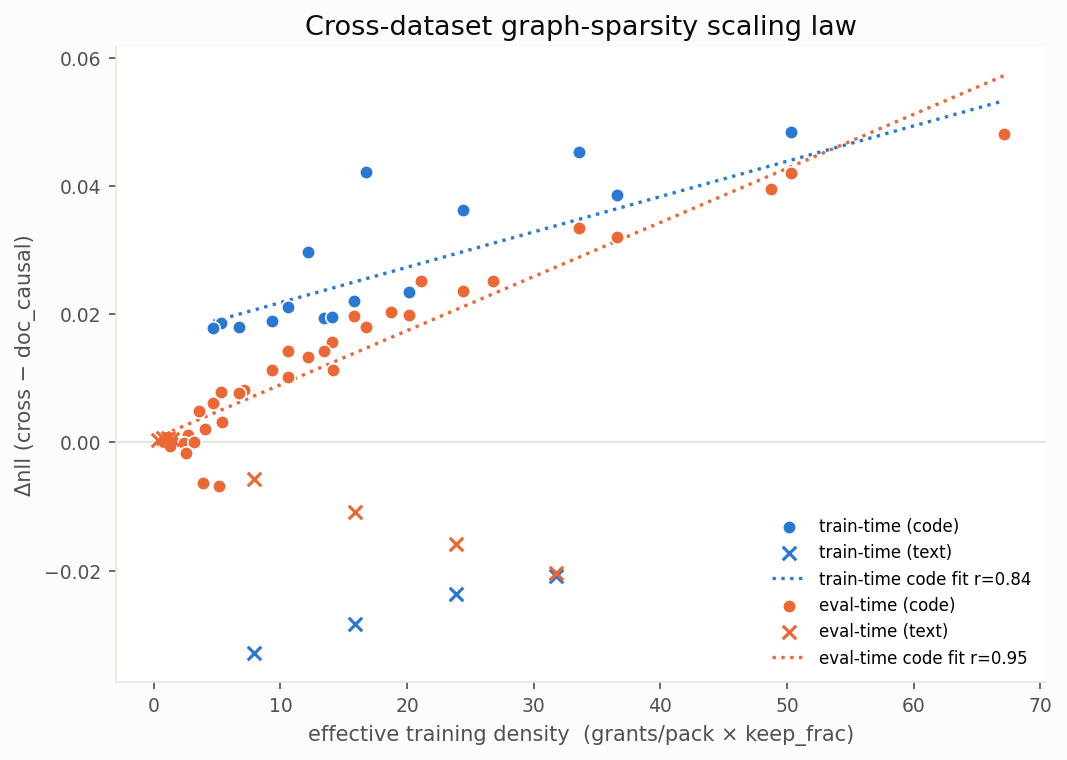
\includegraphics[width=0.72\linewidth]{regression.png}
  \caption{Pooled cross-dataset regression of cross-doc benefit vs effective grant
  density $\times$ keep fraction, train-time (blue) vs eval-time (orange), code
  (circles) vs text (crosses), with code OLS fits.}
  \label{fig:sparsity-regression}
\end{figure}
\begin{itemize}
  \item \textbf{\cref{fig:sparsity-regression}.} The quantitative form of the
  cross-dataset law in \cref{sec:sparsity}, pooling all (dataset, keep) points on the
  honest density axis (effective grants/pack $\times$ keep). \emph{Meaning:} code is
  near-linear both eval-time ($r{=}0.95$) and train-time ($r{=}0.84$); the lower
  train-time $r$ and its positive intercept ($\sim{+}0.016$) reflect the concavity
  (much of the benefit already present at low density). Text datasets sit off the code
  line. Raw graph out-degree is the wrong axis ($r{=}{-}0.27$, a misleading null)
  because it counts edges the mask never used.
\end{itemize}

\subsection{Graph-sparsity: mask-time vs traversal-time validation}
\label{app:sparsity-traversal}
\begin{figure}[t]
  \centering
  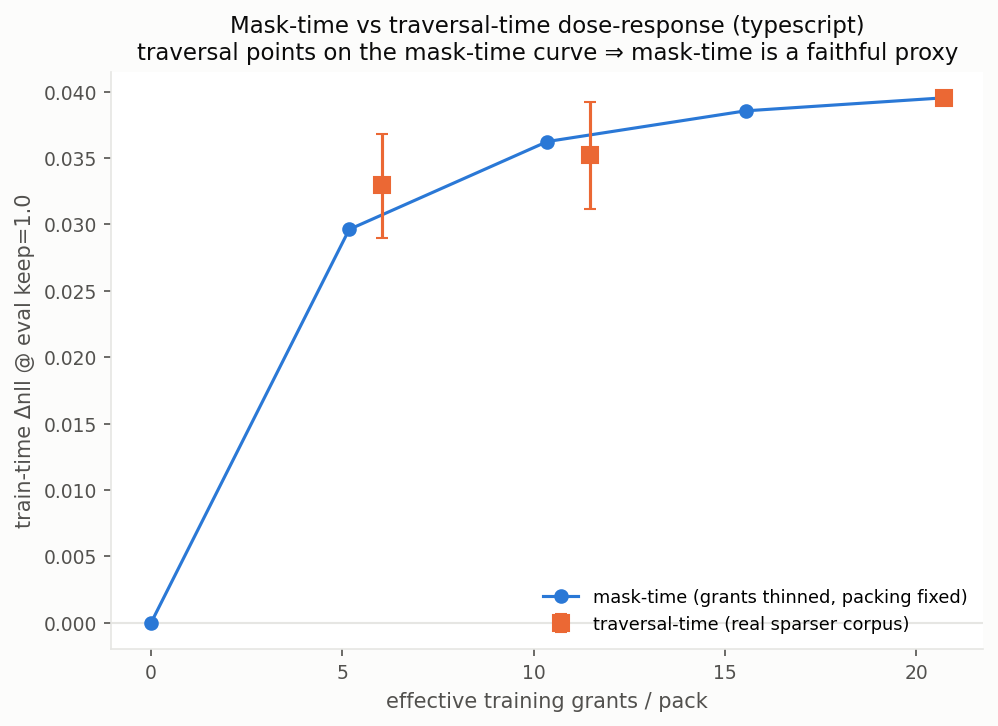
\includegraphics[width=0.62\linewidth]{fig_traversal_check.png}
  \caption{Train-time $\Delta$nll vs effective grant density for \textsc{typescript}:
  cheap \emph{mask-time} dropping (blue, packing fixed) vs \emph{traversal-time}
  dropping (orange, graph adjacency thinned before packing so co-packing itself
  changes --- a genuinely sparser corpus). Error bars are 95\% CIs.}
  \label{fig:sparsity-traversal}
\end{figure}
\begin{itemize}
  \item \textbf{\cref{fig:sparsity-traversal}.} A validity check on the instrument
  behind every density line: does the cheap mask-time subsample (thin recorded grants
  on identical packs) predict the effect of a \emph{really} sparser corpus, where fewer
  links also reshuffle which documents are co-packed? \emph{Meaning:} the traversal-time
  points fall on the mask-time dose-response curve at matched effective density (both
  within CI), so the content-distribution shift from real edge removal does not move the
  curve --- density drives the benefit, and mask-time dropping is a faithful, far
  cheaper proxy.
\end{itemize}



\end{document}
